\originalchapter{8.322公开作业八至十一：表示与散射}
\originalsection{PS8 Q2、Q3：Young表与张量分解}
\begin{exercise}
Q2：画$S_5$所有不可约表示的Young图并计标准表。Q3：列$(\mathbb C^2)^{\otimes5}$、$(\mathbb C^3)^{\otimes4}$在置换群与$SU(2)$或$SU(3)$下的全部表示，并核对维数。
\end{exercise}
\begin{solution}
分拆记号即各行格数。标准表需填$1,\ldots,5$且行列递增；完整图与标准表数如下：
\newcommand{\younggrid}[1]{\begin{tikzpicture}[baseline=(current bounding box.center),x=.22cm,y=.22cm]\foreach \len [count=\row from 0] in {#1}{\foreach \col in {1,...,\len}{\draw (\col,-\row) rectangle ++(-1,-1);}}\end{tikzpicture}}
\begin{center}\begin{tabular}{ccc}
\toprule 分拆 & $f^\lambda$ & Young图\\\midrule
$[5]$&1&\younggrid{5}\\
$[4,1]$&4&\younggrid{4,1}\\
$[3,2]$&5&\younggrid{3,2}\\
$[3,1,1]$&6&\younggrid{3,1,1}\\
$[2,2,1]$&5&\younggrid{2,2,1}\\
$[2,1,1,1]$&4&\younggrid{2,1,1,1}\\
$[1^5]$&1&\younggrid{1,1,1,1,1}\\\bottomrule
\end{tabular}\end{center}

例如$[3,2]$的hook长度为$4,3,1,2,1$，$5!/(4\cdot3\cdot1\cdot2\cdot1)=5$；其余同法。平方和$1+16+25+36+25+16+1=120$，不遗漏不可约表示。

两维内部空间只允许至多两行，故$[5],[4,1],[3,2]$的自旋分别$5/2,3/2,1/2$，置换维数$1,4,5$。分解为$V_{[5]}\otimes D_{5/2}\oplus V_{[4,1]}\otimes D_{3/2}\oplus V_{[3,2]}\otimes D_{1/2}$，$1\cdot6+4\cdot4+5\cdot2=32$。

三维四重张量保$[4],[3,1],[2,2],[2,1,1]$，对应$SU(3)$ Dynkin标号$(4,0),(2,1),(0,2),(1,0)$，维数用$(p+1)(q+1)(p+q+2)/2$分别$15,15,6,3$；置换维数$1,3,2,3$，总计$15+45+12+9=81$。四行图因反对称四个三维向量而零。$[2,1,1]$删三格列成基本表示，但其$S_4$图与维数仍是原来的3，不能一并删去置换结构。
\end{solution}

\originalsection{PS8 Q4、Q5：三电子完整项符号}
\begin{exercise}
Q4：写氮$p^3$构型所有$^2P$波函数。Q5：列$d^3$可能的所有项符号，给空间和自旋的$S_3$表示。
\end{exercise}
\begin{solution}
给$p$壳六个自旋轨道编号$0=(-1,\uparrow),1=(-1,\downarrow),2=(0,\uparrow),3=(0,\downarrow),4=(1,\uparrow),5=(1,\downarrow)$；空间部分为同一径向$R_{np}(r)Y_{1m}(\hat r)$，乘对应自旋函数。定义$D_{abc}=\det[u_a(1),u_b(1),u_c(1);u_a(2),u_b(2),u_c(2);u_a(3),u_b(3),u_c(3)]/\sqrt6$，$a<b<c$，彼此正交归一。全部六个$^2P$态为
\[
\begin{array}{c|cc}
 M_L & M_S=+1/2 & M_S=-1/2\\\hline
 1 &(D_{045}+D_{234})/\sqrt2 &(D_{145}+D_{235})/\sqrt2\\
 0 &(D_{025}-D_{124})/\sqrt2 &(D_{035}-D_{134})/\sqrt2\\
 -1 &(D_{023}+D_{014})/\sqrt2 &(D_{123}+D_{015})/\sqrt2
\end{array}
\]
求法从$M_L=1,M_S=1/2$的两行列式出发，要求$L_+,S_+$湮灭，系数同号；以$L_-/\sqrt2$降$M_L$、$S_-$降$M_S$得表。故最高权$L=1,S=1/2$明确，波函数已完全反对称；不把单个未反对称积叫电子态。$p^3$总20维还含$^4S$四态和$^2D$十态，但本题只要六个$^2P$。

$d^3$的10自旋轨道选3，总维$\binom{10}3=120$。$S=3/2$自旋完全对称$[3]$，空间完全反对称$[1^3]$，$\wedge^3\mathbb C^5$的轨道表示含$L=3,1$，给$^4F,^4P$，维数28+12=40。$S=1/2$自旋$[2,1]$，空间也$[2,1]$，二者取唯一反对称组合；轨道部分的$L=5,4,3,2,2,1$给$^2H,^2G,^2F,2\times{}^2D,^2P$，维数22+18+14+20+6=80。两份$^2D$有不同内部标签，不能合并成一项。此分解另按所有Slater行列式的$(M_L,M_S)$重数作最高权差分复算，120维相合，见数值/符号记录。
\end{solution}

\originalsection{PS8 Q6：质子味--自旋波函数}
\begin{exercise}
求质子$S_z=1/2$的波函数，使三个夸克的味、自旋与颜色满足全同费米要求。
\end{exercise}
\begin{solution}
基态空间对称、颜色单态$\epsilon_{abc}|abc\rangle/\sqrt6$反对称，故味--自旋需完全对称。用三个位置槽写一归一相位约定：
\[
\begin{aligned}
 |p,\uparrow\rangle=\frac1{\sqrt{18}}\{&2|u\uparrow u\uparrow d\downarrow\rangle
 -|u\uparrow u\downarrow d\uparrow\rangle-|u\downarrow u\uparrow d\uparrow\rangle\\
 &+2|u\uparrow d\downarrow u\uparrow\rangle
 -|u\uparrow d\uparrow u\downarrow\rangle-|u\downarrow d\uparrow u\uparrow\rangle\\
 &+2|d\downarrow u\uparrow u\uparrow\rangle
 -|d\uparrow u\uparrow u\downarrow\rangle-|d\uparrow u\downarrow u\uparrow\rangle\}.
\end{aligned}
\]
九个积态互相正交，系数平方和18。置换槽保持表达式；$S_z=1/2$，作用$S_+$时每种全上态的系数$2-1-1=0$，故自旋是$1/2$最高权，非$3/2$。同理味$isospin$升算符把$d$改成$u$时系数抵消，给$I=1/2,I_z=1/2$。乘颜色及空间部分后总态反对称。这是基态非相对论夸克模型的味--自旋结构，不是QCD质子所有海夸克/胶子成分的完整波函数。
\end{solution}

\originalsection{PS9 Q1、Q3：Green函数与核形状因子}
\begin{exercise}
Q1：证明$G_\pm(r)=-e^{\pm ikr}/(4\pi r)$满足$(\nabla^2+k^2)G_\pm=\delta^3(\vct r)$。Q3：电子由总电荷$Ze$、半径$R$均匀带电球核散射，求第一Born振幅与截面。
\end{exercise}
\begin{solution}
$r\ne0$时直接求径向Laplacian为$-k^2G$。在小球积分，$k^2\int G=O(\epsilon^2)$，表面$4\pi\epsilon^2G'(\epsilon)\to1$，故delta系数+1。加号为出射、负号为入射；单靠局部微分方程不能选择实验边界。

均匀球电荷密度$3Ze/(4\pi R^3)$的Fourier变换为$Ze F(QR)$，$F(z)=3(\sin z-z\cos z)/z^3$、$F(0)=1$。Poisson方程给电子势变换$\widetilde V(Q)=-4\pi ZgF(QR)/Q^2$，$g=e^2/(4\pi\epsilon_0)$。所以
\[
 f_B(\theta)=\frac{2mZg}{\hbar^2Q^2}F(QR),\qquad
 \frac{\dd\sigma}{\dd\Omega}=\frac{4m^2Z^2g^2}{\hbar^4Q^4}|F(QR)|^2,\quad Q=2k\sin(\theta/2).
\]
长程Coulomb的Fourier积分先用$e^{-\varepsilon r}$正则化再在非前向取极限；前向发散不能当普通收敛积分。$QR\ll1$回点核Rutherford；大$QR$形状因子抑制并有衍射零点。非相对论第一Born还要求适用的弱耦合/高能范围，不把核尺度波数所需的高能自动认作非相对论。
\end{solution}

\originalsection{PS10 Q2：平面波与能量角动量态归一}
\begin{exercise}
课堂$e^{ikz}=\sum_l a_lj_l(kr)P_l(\cos\theta)$。(a)求$a_l$；(b)若$\langle\vct p|E,l,m\rangle=g_{lE}(p)Y_{lm}(\hat p)$，求$g_{lE}$。原题只援引课堂公式，需在解答明示连续归一。
\end{exercise}
\begin{solution}
Legendre正交投影给$a_lj_l(z)=(2l+1)\int_{-1}^1e^{izt}P_l(t)\dd t/2$，积分表示$\int e^{izt}P_l(t)\dd t=2i^lj_l(z)$，故$a_l=(2l+1)i^l$。该表示可由$P_l$的Rodrigues式逐次分部积分建立，端点项消失。

选$\langle\vct p|\vct p'\rangle=\delta^3(\vct p-\vct p')$、$\langle E,l,m|E',l',m'\rangle=\delta(E-E')\delta_{ll'}\delta_{mm'}$，$p_E=\sqrt{2mE}$。固定能量迫使$g=C_E\delta(p-p_E)$；积分$p^2\dd p$并用$\delta(p_E-p_{E'})=(p_E/m)\delta(E-E')$给$|C_E|=\sqrt{m/p_E^3}$。选位置径向为实正的小$r$相位，
\[
 g_{lE}(p)=(-i)^l\sqrt{\frac m{p_E^3}}\delta(p-p_E),\qquad
 \langle\vct r|E,l,m\rangle=\sqrt{\frac{2mp_E}{\pi\hbar^3}}
 j_l(p_Er/\hbar)Y_{lm}(\hat r).
\]
它由$(2\pi\hbar)^{-3/2}$Fourier核和球谐加法定理得出。若采用动量大小归一而非能量归一，前因子改变；原题未写这一约定，不能把课堂的未知规范化强行当唯一答案。
\end{solution}

\originalsection{PS11 Q1：硬球完整数值图}
\begin{exercise}
硬球半径$R$，(a)画$|f(\theta)|^2$对$\theta$，$\rho=kR=0.1,0.5,1,10,25,100$；(b)画$\sigma_{\rm tot}/(\pi R^2)$，$\rho\le100$。
\end{exercise}
\begin{solution}
边界$u_l(R)=0$给$\tan\delta_l=j_l(\rho)/n_l(\rho)$。数值避免反三角分支，直接取$e^{i\delta_l}\sin\delta_l=j_l/(n_l-ij_l)$；求$f/R=\rho^{-1}\sum_l(2l+1)j_lP_l/(n_l-ij_l)$。取$l_{\max}=\lceil\rho+4\rho^{1/3}+14\rceil$，高于有效冲量参数范围；角度601点、总截面1001点，并以低能4、高能2、尾项收敛和总角积分检查。下图按$R^2$缩放，故适用于任意半径，不另取未知$R$。
\begin{figure}[htbp]\centering
\begin{tikzpicture}\begin{semilogyaxis}[width=.94\textwidth,height=6cm,xlabel={$\theta$（度）},ylabel={$|f/R|^2$},xmin=0,xmax=180,legend columns=3,legend style={font=\small},ymin=1e-6]
\addplot+[no marks] coordinates {(0.000,1.016541) (0.300,1.016541) (0.600,1.01654) (0.900,1.016539) (1.200,1.016537) (1.500,1.016535) (1.800,1.016532) (2.100,1.016528) (2.400,1.016524) (2.700,1.016519) (3.000,1.016514) (3.300,1.016508) (3.600,1.016502) (3.900,1.016495) (4.200,1.016488) (4.500,1.01648) (4.800,1.016471) (5.100,1.016462) (5.400,1.016453) (5.700,1.016442) (6.000,1.016432) (6.300,1.016421) (6.600,1.016409) (6.900,1.016396) (7.200,1.016384) (7.500,1.01637) (7.800,1.016356) (8.100,1.016342) (8.400,1.016327) (8.700,1.016311) (9.000,1.016295) (9.300,1.016278) (9.600,1.016261) (9.900,1.016243) (10.200,1.016225) (10.500,1.016206) (10.800,1.016187) (11.100,1.016167) (11.400,1.016147) (11.700,1.016126) (12.000,1.016104) (12.300,1.016082) (12.600,1.016059) (12.900,1.016036) (13.200,1.016013) (13.500,1.015989) (13.800,1.015964) (14.100,1.015939) (14.400,1.015913) (14.700,1.015886) (15.000,1.01586) (15.300,1.015832) (15.600,1.015804) (15.900,1.015776) (16.200,1.015747) (16.500,1.015717) (16.800,1.015687) (17.100,1.015657) (17.400,1.015626) (17.700,1.015594) (18.000,1.015562) (18.300,1.01553) (18.600,1.015496) (18.900,1.015463) (19.200,1.015429) (19.500,1.015394) (19.800,1.015359) (20.100,1.015323) (20.400,1.015287) (20.700,1.01525) (21.000,1.015213) (21.300,1.015175) (21.600,1.015137) (21.900,1.015098) (22.200,1.015059) (22.500,1.015019) (22.800,1.014978) (23.100,1.014938) (23.400,1.014896) (23.700,1.014854) (24.000,1.014812) (24.300,1.014769) (24.600,1.014726) (24.900,1.014682) (25.200,1.014638) (25.500,1.014593) (25.800,1.014548) (26.100,1.014502) (26.400,1.014456) (26.700,1.014409) (27.000,1.014362) (27.300,1.014314) (27.600,1.014266) (27.900,1.014217) (28.200,1.014168) (28.500,1.014118) (28.800,1.014068) (29.100,1.014017) (29.400,1.013966) (29.700,1.013915) (30.000,1.013862) (30.300,1.01381) (30.600,1.013757) (30.900,1.013703) (31.200,1.013649) (31.500,1.013595) (31.800,1.01354) (32.100,1.013485) (32.400,1.013429) (32.700,1.013373) (33.000,1.013316) (33.300,1.013259) (33.600,1.013201) (33.900,1.013143) (34.200,1.013085) (34.500,1.013026) (34.800,1.012966) (35.100,1.012906) (35.400,1.012846) (35.700,1.012785) (36.000,1.012724) (36.300,1.012662) (36.600,1.0126) (36.900,1.012538) (37.200,1.012475) (37.500,1.012411) (37.800,1.012347) (38.100,1.012283) (38.400,1.012218) (38.700,1.012153) (39.000,1.012088) (39.300,1.012022) (39.600,1.011955) (39.900,1.011889) (40.200,1.011821) (40.500,1.011754) (40.800,1.011686) (41.100,1.011617) (41.400,1.011548) (41.700,1.011479) (42.000,1.01141) (42.300,1.011339) (42.600,1.011269) (42.900,1.011198) (43.200,1.011127) (43.500,1.011055) (43.800,1.010983) (44.100,1.010911) (44.400,1.010838) (44.700,1.010764) (45.000,1.010691) (45.300,1.010617) (45.600,1.010542) (45.900,1.010468) (46.200,1.010393) (46.500,1.010317) (46.800,1.010241) (47.100,1.010165) (47.400,1.010088) (47.700,1.010011) (48.000,1.009934) (48.300,1.009856) (48.600,1.009778) (48.900,1.0097) (49.200,1.009621) (49.500,1.009542) (49.800,1.009462) (50.100,1.009382) (50.400,1.009302) (50.700,1.009222) (51.000,1.009141) (51.300,1.00906) (51.600,1.008978) (51.900,1.008896) (52.200,1.008814) (52.500,1.008732) (52.800,1.008649) (53.100,1.008565) (53.400,1.008482) (53.700,1.008398) (54.000,1.008314) (54.300,1.008229) (54.600,1.008145) (54.900,1.00806) (55.200,1.007974) (55.500,1.007888) (55.800,1.007802) (56.100,1.007716) (56.400,1.00763) (56.700,1.007543) (57.000,1.007455) (57.300,1.007368) (57.600,1.00728) (57.900,1.007192) (58.200,1.007104) (58.500,1.007015) (58.800,1.006926) (59.100,1.006837) (59.400,1.006747) (59.700,1.006658) (60.000,1.006568) (60.300,1.006477) (60.600,1.006387) (60.900,1.006296) (61.200,1.006205) (61.500,1.006114) (61.800,1.006022) (62.100,1.00593) (62.400,1.005838) (62.700,1.005746) (63.000,1.005653) (63.300,1.00556) (63.600,1.005467) (63.900,1.005374) (64.200,1.005281) (64.500,1.005187) (64.800,1.005093) (65.100,1.004999) (65.400,1.004904) (65.700,1.004809) (66.000,1.004715) (66.300,1.00462) (66.600,1.004524) (66.900,1.004429) (67.200,1.004333) (67.500,1.004237) (67.800,1.004141) (68.100,1.004045) (68.400,1.003948) (68.700,1.003851) (69.000,1.003754) (69.300,1.003657) (69.600,1.00356) (69.900,1.003463) (70.200,1.003365) (70.500,1.003267) (70.800,1.003169) (71.100,1.003071) (71.400,1.002973) (71.700,1.002874) (72.000,1.002776) (72.300,1.002677) (72.600,1.002578) (72.900,1.002479) (73.200,1.002379) (73.500,1.00228) (73.800,1.00218) (74.100,1.00208) (74.400,1.001981) (74.700,1.001881) (75.000,1.00178) (75.300,1.00168) (75.600,1.00158) (75.900,1.001479) (76.200,1.001378) (76.500,1.001278) (76.800,1.001177) (77.100,1.001076) (77.400,1.000975) (77.700,1.000873) (78.000,1.000772) (78.300,1.00067) (78.600,1.000569) (78.900,1.000467) (79.200,1.000365) (79.500,1.000263) (79.800,1.000161) (80.100,1.000059) (80.400,0.9999573) (80.700,0.9998551) (81.000,0.9997528) (81.300,0.9996504) (81.600,0.9995479) (81.900,0.9994454) (82.200,0.9993428) (82.500,0.9992401) (82.800,0.9991374) (83.100,0.9990346) (83.400,0.9989317) (83.700,0.9988288) (84.000,0.9987259) (84.300,0.9986229) (84.600,0.9985198) (84.900,0.9984167) (85.200,0.9983136) (85.500,0.9982104) (85.800,0.9981072) (86.100,0.9980039) (86.400,0.9979007) (86.700,0.9977974) (87.000,0.997694) (87.300,0.9975907) (87.600,0.9974873) (87.900,0.997384) (88.200,0.9972806) (88.500,0.9971772) (88.800,0.9970737) (89.100,0.9969703) (89.400,0.9968669) (89.700,0.9967635) (90.000,0.9966601) (90.300,0.9965567) (90.600,0.9964533) (90.900,0.9963499) (91.200,0.9962466) (91.500,0.9961432) (91.800,0.9960399) (92.100,0.9959366) (92.400,0.9958333) (92.700,0.9957301) (93.000,0.9956269) (93.300,0.9955237) (93.600,0.9954206) (93.900,0.9953175) (94.200,0.9952144) (94.500,0.9951114) (94.800,0.9950085) (95.100,0.9949056) (95.400,0.9948027) (95.700,0.9946999) (96.000,0.9945972) (96.300,0.9944945) (96.600,0.9943919) (96.900,0.9942894) (97.200,0.9941869) (97.500,0.9940846) (97.800,0.9939823) (98.100,0.99388) (98.400,0.9937779) (98.700,0.9936758) (99.000,0.9935739) (99.300,0.993472) (99.600,0.9933702) (99.900,0.9932685) (100.200,0.993167) (100.500,0.9930655) (100.800,0.9929641) (101.100,0.9928628) (101.400,0.9927617) (101.700,0.9926606) (102.000,0.9925597) (102.300,0.9924589) (102.600,0.9923582) (102.900,0.9922577) (103.200,0.9921572) (103.500,0.9920569) (103.800,0.9919568) (104.100,0.9918567) (104.400,0.9917568) (104.700,0.9916571) (105.000,0.9915575) (105.300,0.991458) (105.600,0.9913587) (105.900,0.9912595) (106.200,0.9911605) (106.500,0.9910617) (106.800,0.990963) (107.100,0.9908645) (107.400,0.9907661) (107.700,0.9906679) (108.000,0.9905699) (108.300,0.990472) (108.600,0.9903743) (108.900,0.9902768) (109.200,0.9901795) (109.500,0.9900824) (109.800,0.9899854) (110.100,0.9898887) (110.400,0.9897921) (110.700,0.9896957) (111.000,0.9895996) (111.300,0.9895036) (111.600,0.9894078) (111.900,0.9893122) (112.200,0.9892169) (112.500,0.9891217) (112.800,0.9890268) (113.100,0.9889321) (113.400,0.9888376) (113.700,0.9887433) (114.000,0.9886492) (114.300,0.9885554) (114.600,0.9884617) (114.900,0.9883684) (115.200,0.9882752) (115.500,0.9881823) (115.800,0.9880896) (116.100,0.9879972) (116.400,0.987905) (116.700,0.987813) (117.000,0.9877213) (117.300,0.9876299) (117.600,0.9875387) (117.900,0.9874477) (118.200,0.987357) (118.500,0.9872666) (118.800,0.9871765) (119.100,0.9870866) (119.400,0.9869969) (119.700,0.9869076) (120.000,0.9868185) (120.300,0.9867296) (120.600,0.9866411) (120.900,0.9865528) (121.200,0.9864649) (121.500,0.9863772) (121.800,0.9862897) (122.100,0.9862026) (122.400,0.9861158) (122.700,0.9860293) (123.000,0.985943) (123.300,0.9858571) (123.600,0.9857714) (123.900,0.9856861) (124.200,0.985601) (124.500,0.9855163) (124.800,0.9854319) (125.100,0.9853478) (125.400,0.985264) (125.700,0.9851805) (126.000,0.9850973) (126.300,0.9850145) (126.600,0.984932) (126.900,0.9848498) (127.200,0.9847679) (127.500,0.9846864) (127.800,0.9846052) (128.100,0.9845243) (128.400,0.9844438) (128.700,0.9843636) (129.000,0.9842837) (129.300,0.9842042) (129.600,0.984125) (129.900,0.9840462) (130.200,0.9839677) (130.500,0.9838896) (130.800,0.9838118) (131.100,0.9837344) (131.400,0.9836573) (131.700,0.9835806) (132.000,0.9835043) (132.300,0.9834283) (132.600,0.9833527) (132.900,0.9832775) (133.200,0.9832026) (133.500,0.9831281) (133.800,0.9830539) (134.100,0.9829802) (134.400,0.9829068) (134.700,0.9828338) (135.000,0.9827612) (135.300,0.9826889) (135.600,0.9826171) (135.900,0.9825456) (136.200,0.9824745) (136.500,0.9824038) (136.800,0.9823335) (137.100,0.9822636) (137.400,0.9821941) (137.700,0.982125) (138.000,0.9820563) (138.300,0.981988) (138.600,0.9819201) (138.900,0.9818526) (139.200,0.9817855) (139.500,0.9817188) (139.800,0.9816526) (140.100,0.9815867) (140.400,0.9815213) (140.700,0.9814562) (141.000,0.9813916) (141.300,0.9813274) (141.600,0.9812637) (141.900,0.9812003) (142.200,0.9811374) (142.500,0.9810749) (142.800,0.9810128) (143.100,0.9809512) (143.400,0.98089) (143.700,0.9808292) (144.000,0.9807688) (144.300,0.9807089) (144.600,0.9806495) (144.900,0.9805904) (145.200,0.9805318) (145.500,0.9804737) (145.800,0.980416) (146.100,0.9803587) (146.400,0.9803019) (146.700,0.9802455) (147.000,0.9801896) (147.300,0.9801342) (147.600,0.9800792) (147.900,0.9800246) (148.200,0.9799705) (148.500,0.9799168) (148.800,0.9798637) (149.100,0.9798109) (149.400,0.9797587) (149.700,0.9797069) (150.000,0.9796555) (150.300,0.9796046) (150.600,0.9795542) (150.900,0.9795043) (151.200,0.9794548) (151.500,0.9794058) (151.800,0.9793573) (152.100,0.9793092) (152.400,0.9792617) (152.700,0.9792146) (153.000,0.9791679) (153.300,0.9791218) (153.600,0.9790761) (153.900,0.9790309) (154.200,0.9789862) (154.500,0.978942) (154.800,0.9788983) (155.100,0.978855) (155.400,0.9788122) (155.700,0.9787699) (156.000,0.9787282) (156.300,0.9786869) (156.600,0.978646) (156.900,0.9786057) (157.200,0.9785659) (157.500,0.9785266) (157.800,0.9784877) (158.100,0.9784494) (158.400,0.9784115) (158.700,0.9783742) (159.000,0.9783373) (159.300,0.978301) (159.600,0.9782651) (159.900,0.9782298) (160.200,0.978195) (160.500,0.9781606) (160.800,0.9781268) (161.100,0.9780935) (161.400,0.9780606) (161.700,0.9780283) (162.000,0.9779965) (162.300,0.9779652) (162.600,0.9779344) (162.900,0.9779042) (163.200,0.9778744) (163.500,0.9778452) (163.800,0.9778164) (164.100,0.9777882) (164.400,0.9777605) (164.700,0.9777333) (165.000,0.9777066) (165.300,0.9776805) (165.600,0.9776548) (165.900,0.9776297) (166.200,0.9776051) (166.500,0.977581) (166.800,0.9775574) (167.100,0.9775344) (167.400,0.9775119) (167.700,0.9774899) (168.000,0.9774684) (168.300,0.9774474) (168.600,0.977427) (168.900,0.9774071) (169.200,0.9773877) (169.500,0.9773688) (169.800,0.9773505) (170.100,0.9773327) (170.400,0.9773154) (170.700,0.9772986) (171.000,0.9772824) (171.300,0.9772667) (171.600,0.9772515) (171.900,0.9772369) (172.200,0.9772228) (172.500,0.9772092) (172.800,0.9771961) (173.100,0.9771836) (173.400,0.9771716) (173.700,0.9771602) (174.000,0.9771492) (174.300,0.9771388) (174.600,0.977129) (174.900,0.9771196) (175.200,0.9771108) (175.500,0.9771026) (175.800,0.9770948) (176.100,0.9770876) (176.400,0.9770809) (176.700,0.9770748) (177.000,0.9770692) (177.300,0.9770641) (177.600,0.9770596) (177.900,0.9770556) (178.200,0.9770521) (178.500,0.9770492) (178.800,0.9770468) (179.100,0.9770449) (179.400,0.9770435) (179.700,0.9770427) (180.000,0.9770425)};
\addlegendentry{$kR=0.1$}
\addplot+[no marks] coordinates {(0.000,1.355017) (0.300,1.35501) (0.600,1.354989) (0.900,1.354953) (1.200,1.354904) (1.500,1.35484) (1.800,1.354763) (2.100,1.354671) (2.400,1.354565) (2.700,1.354446) (3.000,1.354312) (3.300,1.354164) (3.600,1.354001) (3.900,1.353825) (4.200,1.353635) (4.500,1.353431) (4.800,1.353213) (5.100,1.35298) (5.400,1.352734) (5.700,1.352474) (6.000,1.3522) (6.300,1.351911) (6.600,1.351609) (6.900,1.351293) (7.200,1.350963) (7.500,1.350619) (7.800,1.350262) (8.100,1.34989) (8.400,1.349505) (8.700,1.349105) (9.000,1.348692) (9.300,1.348265) (9.600,1.347825) (9.900,1.34737) (10.200,1.346902) (10.500,1.346421) (10.800,1.345925) (11.100,1.345416) (11.400,1.344893) (11.700,1.344357) (12.000,1.343807) (12.300,1.343244) (12.600,1.342667) (12.900,1.342077) (13.200,1.341473) (13.500,1.340856) (13.800,1.340226) (14.100,1.339582) (14.400,1.338925) (14.700,1.338254) (15.000,1.337571) (15.300,1.336874) (15.600,1.336164) (15.900,1.335441) (16.200,1.334705) (16.500,1.333955) (16.800,1.333193) (17.100,1.332418) (17.400,1.33163) (17.700,1.330828) (18.000,1.330015) (18.300,1.329188) (18.600,1.328348) (18.900,1.327496) (19.200,1.326631) (19.500,1.325753) (19.800,1.324863) (20.100,1.323961) (20.400,1.323045) (20.700,1.322118) (21.000,1.321178) (21.300,1.320225) (21.600,1.31926) (21.900,1.318283) (22.200,1.317294) (22.500,1.316293) (22.800,1.315279) (23.100,1.314254) (23.400,1.313216) (23.700,1.312167) (24.000,1.311105) (24.300,1.310032) (24.600,1.308947) (24.900,1.30785) (25.200,1.306741) (25.500,1.305621) (25.800,1.30449) (26.100,1.303346) (26.400,1.302192) (26.700,1.301025) (27.000,1.299848) (27.300,1.298659) (27.600,1.297459) (27.900,1.296248) (28.200,1.295026) (28.500,1.293792) (28.800,1.292548) (29.100,1.291293) (29.400,1.290027) (29.700,1.28875) (30.000,1.287462) (30.300,1.286164) (30.600,1.284855) (30.900,1.283536) (31.200,1.282206) (31.500,1.280865) (31.800,1.279515) (32.100,1.278154) (32.400,1.276782) (32.700,1.275401) (33.000,1.274009) (33.300,1.272608) (33.600,1.271196) (33.900,1.269775) (34.200,1.268344) (34.500,1.266903) (34.800,1.265452) (35.100,1.263992) (35.400,1.262522) (35.700,1.261043) (36.000,1.259555) (36.300,1.258057) (36.600,1.25655) (36.900,1.255033) (37.200,1.253508) (37.500,1.251973) (37.800,1.25043) (38.100,1.248877) (38.400,1.247316) (38.700,1.245746) (39.000,1.244167) (39.300,1.24258) (39.600,1.240984) (39.900,1.23938) (40.200,1.237767) (40.500,1.236147) (40.800,1.234517) (41.100,1.23288) (41.400,1.231235) (41.700,1.229581) (42.000,1.22792) (42.300,1.226251) (42.600,1.224574) (42.900,1.222889) (43.200,1.221197) (43.500,1.219497) (43.800,1.21779) (44.100,1.216075) (44.400,1.214353) (44.700,1.212624) (45.000,1.210888) (45.300,1.209144) (45.600,1.207394) (45.900,1.205637) (46.200,1.203872) (46.500,1.202101) (46.800,1.200324) (47.100,1.198539) (47.400,1.196749) (47.700,1.194951) (48.000,1.193148) (48.300,1.191338) (48.600,1.189522) (48.900,1.1877) (49.200,1.185871) (49.500,1.184037) (49.800,1.182197) (50.100,1.180351) (50.400,1.178499) (50.700,1.176642) (51.000,1.174779) (51.300,1.17291) (51.600,1.171037) (51.900,1.169157) (52.200,1.167273) (52.500,1.165383) (52.800,1.163489) (53.100,1.161589) (53.400,1.159684) (53.700,1.157775) (54.000,1.15586) (54.300,1.153941) (54.600,1.152018) (54.900,1.15009) (55.200,1.148157) (55.500,1.14622) (55.800,1.144279) (56.100,1.142333) (56.400,1.140384) (56.700,1.13843) (57.000,1.136472) (57.300,1.134511) (57.600,1.132545) (57.900,1.130576) (58.200,1.128604) (58.500,1.126627) (58.800,1.124647) (59.100,1.122664) (59.400,1.120677) (59.700,1.118688) (60.000,1.116694) (60.300,1.114698) (60.600,1.112699) (60.900,1.110697) (61.200,1.108692) (61.500,1.106684) (61.800,1.104673) (62.100,1.10266) (62.400,1.100644) (62.700,1.098626) (63.000,1.096605) (63.300,1.094582) (63.600,1.092557) (63.900,1.09053) (64.200,1.0885) (64.500,1.086469) (64.800,1.084435) (65.100,1.0824) (65.400,1.080363) (65.700,1.078324) (66.000,1.076283) (66.300,1.074241) (66.600,1.072197) (66.900,1.070152) (67.200,1.068106) (67.500,1.066058) (67.800,1.06401) (68.100,1.06196) (68.400,1.059909) (68.700,1.057857) (69.000,1.055804) (69.300,1.05375) (69.600,1.051695) (69.900,1.04964) (70.200,1.047584) (70.500,1.045528) (70.800,1.043471) (71.100,1.041414) (71.400,1.039357) (71.700,1.037299) (72.000,1.035241) (72.300,1.033183) (72.600,1.031124) (72.900,1.029066) (73.200,1.027008) (73.500,1.02495) (73.800,1.022893) (74.100,1.020836) (74.400,1.018779) (74.700,1.016722) (75.000,1.014666) (75.300,1.012611) (75.600,1.010556) (75.900,1.008502) (76.200,1.006448) (76.500,1.004396) (76.800,1.002344) (77.100,1.000294) (77.400,0.998244) (77.700,0.9961955) (78.000,0.9941481) (78.300,0.992102) (78.600,0.9900572) (78.900,0.9880138) (79.200,0.9859717) (79.500,0.9839311) (79.800,0.9818921) (80.100,0.9798547) (80.400,0.977819) (80.700,0.975785) (81.000,0.9737527) (81.300,0.9717224) (81.600,0.9696939) (81.900,0.9676674) (82.200,0.965643) (82.500,0.9636206) (82.800,0.9616004) (83.100,0.9595824) (83.400,0.9575666) (83.700,0.9555532) (84.000,0.9535422) (84.300,0.9515336) (84.600,0.9495275) (84.900,0.9475239) (85.200,0.945523) (85.500,0.9435247) (85.800,0.9415292) (86.100,0.9395364) (86.400,0.9375464) (86.700,0.9355594) (87.000,0.9335753) (87.300,0.9315941) (87.600,0.929616) (87.900,0.927641) (88.200,0.9256692) (88.500,0.9237006) (88.800,0.9217352) (89.100,0.9197731) (89.400,0.9178144) (89.700,0.915859) (90.000,0.9139072) (90.300,0.9119588) (90.600,0.910014) (90.900,0.9080728) (91.200,0.9061353) (91.500,0.9042014) (91.800,0.9022713) (92.100,0.900345) (92.400,0.8984226) (92.700,0.896504) (93.000,0.8945894) (93.300,0.8926787) (93.600,0.8907721) (93.900,0.8888695) (94.200,0.8869711) (94.500,0.8850768) (94.800,0.8831868) (95.100,0.881301) (95.400,0.8794194) (95.700,0.8775423) (96.000,0.8756695) (96.300,0.8738011) (96.600,0.8719371) (96.900,0.8700777) (97.200,0.8682228) (97.500,0.8663726) (97.800,0.8645269) (98.100,0.8626859) (98.400,0.8608496) (98.700,0.859018) (99.000,0.8571913) (99.300,0.8553693) (99.600,0.8535522) (99.900,0.85174) (100.200,0.8499328) (100.500,0.8481305) (100.800,0.8463332) (101.100,0.8445409) (101.400,0.8427537) (101.700,0.8409717) (102.000,0.8391948) (102.300,0.8374231) (102.600,0.8356565) (102.900,0.8338953) (103.200,0.8321393) (103.500,0.8303887) (103.800,0.8286433) (104.100,0.8269034) (104.400,0.8251689) (104.700,0.8234398) (105.000,0.8217163) (105.300,0.8199982) (105.600,0.8182856) (105.900,0.8165787) (106.200,0.8148773) (106.500,0.8131815) (106.800,0.8114915) (107.100,0.8098071) (107.400,0.8081284) (107.700,0.8064554) (108.000,0.8047882) (108.300,0.8031269) (108.600,0.8014713) (108.900,0.7998216) (109.200,0.7981778) (109.500,0.7965399) (109.800,0.7949079) (110.100,0.7932819) (110.400,0.7916618) (110.700,0.7900478) (111.000,0.7884398) (111.300,0.7868378) (111.600,0.7852419) (111.900,0.7836522) (112.200,0.7820685) (112.500,0.780491) (112.800,0.7789197) (113.100,0.7773545) (113.400,0.7757956) (113.700,0.7742429) (114.000,0.7726964) (114.300,0.7711563) (114.600,0.7696224) (114.900,0.7680949) (115.200,0.7665737) (115.500,0.7650588) (115.800,0.7635503) (116.100,0.7620483) (116.400,0.7605526) (116.700,0.7590634) (117.000,0.7575806) (117.300,0.7561043) (117.600,0.7546345) (117.900,0.7531712) (118.200,0.7517144) (118.500,0.7502641) (118.800,0.7488204) (119.100,0.7473833) (119.400,0.7459528) (119.700,0.7445288) (120.000,0.7431115) (120.300,0.7417008) (120.600,0.7402968) (120.900,0.7388994) (121.200,0.7375087) (121.500,0.7361247) (121.800,0.7347474) (122.100,0.7333769) (122.400,0.732013) (122.700,0.7306559) (123.000,0.7293056) (123.300,0.727962) (123.600,0.7266252) (123.900,0.7252952) (124.200,0.723972) (124.500,0.7226557) (124.800,0.7213461) (125.100,0.7200434) (125.400,0.7187476) (125.700,0.7174586) (126.000,0.7161765) (126.300,0.7149013) (126.600,0.713633) (126.900,0.7123715) (127.200,0.711117) (127.500,0.7098694) (127.800,0.7086288) (128.100,0.7073951) (128.400,0.7061683) (128.700,0.7049485) (129.000,0.7037356) (129.300,0.7025298) (129.600,0.7013309) (129.900,0.700139) (130.200,0.6989541) (130.500,0.6977762) (130.800,0.6966053) (131.100,0.6954414) (131.400,0.6942846) (131.700,0.6931348) (132.000,0.691992) (132.300,0.6908562) (132.600,0.6897276) (132.900,0.6886059) (133.200,0.6874914) (133.500,0.6863839) (133.800,0.6852835) (134.100,0.6841901) (134.400,0.6831039) (134.700,0.6820247) (135.000,0.6809526) (135.300,0.6798876) (135.600,0.6788297) (135.900,0.677779) (136.200,0.6767353) (136.500,0.6756987) (136.800,0.6746693) (137.100,0.673647) (137.400,0.6726318) (137.700,0.6716237) (138.000,0.6706228) (138.300,0.669629) (138.600,0.6686423) (138.900,0.6676628) (139.200,0.6666904) (139.500,0.6657252) (139.800,0.6647671) (140.100,0.6638162) (140.400,0.6628724) (140.700,0.6619358) (141.000,0.6610063) (141.300,0.660084) (141.600,0.6591688) (141.900,0.6582608) (142.200,0.65736) (142.500,0.6564663) (142.800,0.6555798) (143.100,0.6547005) (143.400,0.6538283) (143.700,0.6529633) (144.000,0.6521055) (144.300,0.6512549) (144.600,0.6504114) (144.900,0.6495751) (145.200,0.6487459) (145.500,0.647924) (145.800,0.6471092) (146.100,0.6463015) (146.400,0.6455011) (146.700,0.6447078) (147.000,0.6439217) (147.300,0.6431428) (147.600,0.6423711) (147.900,0.6416065) (148.200,0.6408491) (148.500,0.6400989) (148.800,0.6393558) (149.100,0.6386199) (149.400,0.6378912) (149.700,0.6371697) (150.000,0.6364553) (150.300,0.6357481) (150.600,0.6350481) (150.900,0.6343552) (151.200,0.6336696) (151.500,0.632991) (151.800,0.6323197) (152.100,0.6316555) (152.400,0.6309985) (152.700,0.6303486) (153.000,0.6297059) (153.300,0.6290704) (153.600,0.628442) (153.900,0.6278208) (154.200,0.6272068) (154.500,0.6265999) (154.800,0.6260001) (155.100,0.6254076) (155.400,0.6248221) (155.700,0.6242438) (156.000,0.6236727) (156.300,0.6231087) (156.600,0.6225519) (156.900,0.6220022) (157.200,0.6214597) (157.500,0.6209243) (157.800,0.620396) (158.100,0.6198749) (158.400,0.6193609) (158.700,0.6188541) (159.000,0.6183544) (159.300,0.6178618) (159.600,0.6173764) (159.900,0.616898) (160.200,0.6164269) (160.500,0.6159628) (160.800,0.6155059) (161.100,0.6150561) (161.400,0.6146134) (161.700,0.6141779) (162.000,0.6137494) (162.300,0.6133281) (162.600,0.6129139) (162.900,0.6125068) (163.200,0.6121068) (163.500,0.611714) (163.800,0.6113282) (164.100,0.6109496) (164.400,0.6105781) (164.700,0.6102136) (165.000,0.6098563) (165.300,0.6095061) (165.600,0.609163) (165.900,0.6088269) (166.200,0.608498) (166.500,0.6081762) (166.800,0.6078615) (167.100,0.6075538) (167.400,0.6072533) (167.700,0.6069598) (168.000,0.6066735) (168.300,0.6063942) (168.600,0.606122) (168.900,0.6058569) (169.200,0.6055989) (169.500,0.605348) (169.800,0.6051042) (170.100,0.6048674) (170.400,0.6046377) (170.700,0.6044151) (171.000,0.6041996) (171.300,0.6039911) (171.600,0.6037898) (171.900,0.6035955) (172.200,0.6034082) (172.500,0.6032281) (172.800,0.603055) (173.100,0.602889) (173.400,0.6027301) (173.700,0.6025782) (174.000,0.6024334) (174.300,0.6022957) (174.600,0.602165) (174.900,0.6020414) (175.200,0.6019249) (175.500,0.6018154) (175.800,0.601713) (176.100,0.6016177) (176.400,0.6015294) (176.700,0.6014482) (177.000,0.6013741) (177.300,0.601307) (177.600,0.6012469) (177.900,0.601194) (178.200,0.6011481) (178.500,0.6011093) (178.800,0.6010775) (179.100,0.6010528) (179.400,0.6010351) (179.700,0.6010245) (180.000,0.601021)};
\addlegendentry{$kR=0.5$}
\addplot+[no marks] coordinates {(0.000,2.081039) (0.300,2.081007) (0.600,2.08091) (0.900,2.080749) (1.200,2.080523) (1.500,2.080232) (1.800,2.079877) (2.100,2.079458) (2.400,2.078974) (2.700,2.078426) (3.000,2.077814) (3.300,2.077137) (3.600,2.076397) (3.900,2.075592) (4.200,2.074724) (4.500,2.073791) (4.800,2.072795) (5.100,2.071735) (5.400,2.070612) (5.700,2.069425) (6.000,2.068175) (6.300,2.066862) (6.600,2.065485) (6.900,2.064047) (7.200,2.062545) (7.500,2.060981) (7.800,2.059354) (8.100,2.057666) (8.400,2.055915) (8.700,2.054103) (9.000,2.052229) (9.300,2.050294) (9.600,2.048298) (9.900,2.046241) (10.200,2.044123) (10.500,2.041944) (10.800,2.039706) (11.100,2.037407) (11.400,2.035049) (11.700,2.032632) (12.000,2.030155) (12.300,2.027619) (12.600,2.025025) (12.900,2.022372) (13.200,2.019662) (13.500,2.016893) (13.800,2.014067) (14.100,2.011184) (14.400,2.008244) (14.700,2.005248) (15.000,2.002195) (15.300,1.999087) (15.600,1.995923) (15.900,1.992704) (16.200,1.98943) (16.500,1.986102) (16.800,1.982719) (17.100,1.979283) (17.400,1.975793) (17.700,1.972251) (18.000,1.968656) (18.300,1.965008) (18.600,1.961309) (18.900,1.957558) (19.200,1.953757) (19.500,1.949904) (19.800,1.946002) (20.100,1.942049) (20.400,1.938048) (20.700,1.933997) (21.000,1.929898) (21.300,1.92575) (21.600,1.921555) (21.900,1.917313) (22.200,1.913024) (22.500,1.908688) (22.800,1.904307) (23.100,1.89988) (23.400,1.895409) (23.700,1.890892) (24.000,1.886332) (24.300,1.881728) (24.600,1.877081) (24.900,1.872391) (25.200,1.86766) (25.500,1.862886) (25.800,1.858072) (26.100,1.853216) (26.400,1.848321) (26.700,1.843386) (27.000,1.838412) (27.300,1.833398) (27.600,1.828347) (27.900,1.823258) (28.200,1.818132) (28.500,1.812969) (28.800,1.80777) (29.100,1.802536) (29.400,1.797266) (29.700,1.791962) (30.000,1.786623) (30.300,1.781252) (30.600,1.775847) (30.900,1.770409) (31.200,1.76494) (31.500,1.759439) (31.800,1.753907) (32.100,1.748345) (32.400,1.742752) (32.700,1.737131) (33.000,1.731481) (33.300,1.725802) (33.600,1.720096) (33.900,1.714363) (34.200,1.708603) (34.500,1.702817) (34.800,1.697005) (35.100,1.691168) (35.400,1.685307) (35.700,1.679422) (36.000,1.673514) (36.300,1.667582) (36.600,1.661629) (36.900,1.655653) (37.200,1.649657) (37.500,1.64364) (37.800,1.637602) (38.100,1.631545) (38.400,1.625469) (38.700,1.619374) (39.000,1.613262) (39.300,1.607132) (39.600,1.600985) (39.900,1.594821) (40.200,1.588642) (40.500,1.582448) (40.800,1.576238) (41.100,1.570015) (41.400,1.563777) (41.700,1.557527) (42.000,1.551264) (42.300,1.544989) (42.600,1.538702) (42.900,1.532404) (43.200,1.526096) (43.500,1.519778) (43.800,1.51345) (44.100,1.507113) (44.400,1.500767) (44.700,1.494414) (45.000,1.488053) (45.300,1.481686) (45.600,1.475312) (45.900,1.468931) (46.200,1.462546) (46.500,1.456156) (46.800,1.449761) (47.100,1.443362) (47.400,1.43696) (47.700,1.430555) (48.000,1.424147) (48.300,1.417738) (48.600,1.411327) (48.900,1.404915) (49.200,1.398502) (49.500,1.392089) (49.800,1.385677) (50.100,1.379266) (50.400,1.372856) (50.700,1.366448) (51.000,1.360042) (51.300,1.353639) (51.600,1.347238) (51.900,1.340842) (52.200,1.33445) (52.500,1.328062) (52.800,1.321679) (53.100,1.315302) (53.400,1.30893) (53.700,1.302565) (54.000,1.296206) (54.300,1.289854) (54.600,1.28351) (54.900,1.277174) (55.200,1.270846) (55.500,1.264527) (55.800,1.258217) (56.100,1.251916) (56.400,1.245626) (56.700,1.239345) (57.000,1.233076) (57.300,1.226817) (57.600,1.22057) (57.900,1.214335) (58.200,1.208112) (58.500,1.201902) (58.800,1.195705) (59.100,1.189521) (59.400,1.18335) (59.700,1.177194) (60.000,1.171052) (60.300,1.164924) (60.600,1.158812) (60.900,1.152715) (61.200,1.146634) (61.500,1.140569) (61.800,1.13452) (62.100,1.128487) (62.400,1.122472) (62.700,1.116474) (63.000,1.110494) (63.300,1.104531) (63.600,1.098587) (63.900,1.092661) (64.200,1.086754) (64.500,1.080866) (64.800,1.074997) (65.100,1.069147) (65.400,1.063318) (65.700,1.057509) (66.000,1.05172) (66.300,1.045952) (66.600,1.040204) (66.900,1.034478) (67.200,1.028773) (67.500,1.02309) (67.800,1.017428) (68.100,1.011789) (68.400,1.006172) (68.700,1.000577) (69.000,0.995005) (69.300,0.989456) (69.600,0.9839302) (69.900,0.9784278) (70.200,0.9729488) (70.500,0.9674937) (70.800,0.9620624) (71.100,0.9566553) (71.400,0.9512724) (71.700,0.9459141) (72.000,0.9405803) (72.300,0.9352714) (72.600,0.9299875) (72.900,0.9247287) (73.200,0.9194952) (73.500,0.9142872) (73.800,0.9091047) (74.100,0.903948) (74.400,0.8988171) (74.700,0.8937123) (75.000,0.8886336) (75.300,0.8835811) (75.600,0.8785551) (75.900,0.8735556) (76.200,0.8685826) (76.500,0.8636365) (76.800,0.8587171) (77.100,0.8538247) (77.400,0.8489594) (77.700,0.8441212) (78.000,0.8393102) (78.300,0.8345265) (78.600,0.8297702) (78.900,0.8250415) (79.200,0.8203402) (79.500,0.8156666) (79.800,0.8110207) (80.100,0.8064025) (80.400,0.8018122) (80.700,0.7972497) (81.000,0.7927152) (81.300,0.7882086) (81.600,0.7837301) (81.900,0.7792796) (82.200,0.7748573) (82.500,0.7704631) (82.800,0.7660971) (83.100,0.7617593) (83.400,0.7574497) (83.700,0.7531684) (84.000,0.7489153) (84.300,0.7446906) (84.600,0.7404941) (84.900,0.736326) (85.200,0.7321862) (85.500,0.7280747) (85.800,0.7239915) (86.100,0.7199367) (86.400,0.7159101) (86.700,0.7119119) (87.000,0.707942) (87.300,0.7040003) (87.600,0.7000869) (87.900,0.6962018) (88.200,0.6923448) (88.500,0.6885161) (88.800,0.6847155) (89.100,0.680943) (89.400,0.6771987) (89.700,0.6734824) (90.000,0.6697941) (90.300,0.6661338) (90.600,0.6625014) (90.900,0.6588969) (91.200,0.6553202) (91.500,0.6517714) (91.800,0.6482502) (92.100,0.6447567) (92.400,0.6412909) (92.700,0.6378525) (93.000,0.6344417) (93.300,0.6310583) (93.600,0.6277022) (93.900,0.6243734) (94.200,0.6210718) (94.500,0.6177974) (94.800,0.6145499) (95.100,0.6113295) (95.400,0.608136) (95.700,0.6049693) (96.000,0.6018293) (96.300,0.5987159) (96.600,0.5956291) (96.900,0.5925688) (97.200,0.5895348) (97.500,0.5865271) (97.800,0.5835456) (98.100,0.5805901) (98.400,0.5776607) (98.700,0.5747571) (99.000,0.5718793) (99.300,0.5690272) (99.600,0.5662006) (99.900,0.5633996) (100.200,0.5606238) (100.500,0.5578734) (100.800,0.5551481) (101.100,0.5524477) (101.400,0.5497724) (101.700,0.5471218) (102.000,0.5444959) (102.300,0.5418945) (102.600,0.5393176) (102.900,0.536765) (103.200,0.5342367) (103.500,0.5317324) (103.800,0.5292521) (104.100,0.5267956) (104.400,0.5243629) (104.700,0.5219537) (105.000,0.519568) (105.300,0.5172056) (105.600,0.5148665) (105.900,0.5125504) (106.200,0.5102573) (106.500,0.507987) (106.800,0.5057393) (107.100,0.5035143) (107.400,0.5013116) (107.700,0.4991313) (108.000,0.4969731) (108.300,0.4948369) (108.600,0.4927226) (108.900,0.4906301) (109.200,0.4885591) (109.500,0.4865097) (109.800,0.4844816) (110.100,0.4824747) (110.400,0.4804888) (110.700,0.4785239) (111.000,0.4765798) (111.300,0.4746563) (111.600,0.4727533) (111.900,0.4708707) (112.200,0.4690083) (112.500,0.467166) (112.800,0.4653437) (113.100,0.4635411) (113.400,0.4617583) (113.700,0.4599949) (114.000,0.458251) (114.300,0.4565263) (114.600,0.4548206) (114.900,0.453134) (115.200,0.4514662) (115.500,0.449817) (115.800,0.4481864) (116.100,0.4465741) (116.400,0.4449802) (116.700,0.4434043) (117.000,0.4418464) (117.300,0.4403064) (117.600,0.438784) (117.900,0.4372792) (118.200,0.4357917) (118.500,0.4343216) (118.800,0.4328686) (119.100,0.4314325) (119.400,0.4300133) (119.700,0.4286108) (120.000,0.4272249) (120.300,0.4258554) (120.600,0.4245022) (120.900,0.4231652) (121.200,0.4218441) (121.500,0.420539) (121.800,0.4192495) (122.100,0.4179757) (122.400,0.4167173) (122.700,0.4154743) (123.000,0.4142464) (123.300,0.4130336) (123.600,0.4118357) (123.900,0.4106527) (124.200,0.4094842) (124.500,0.4083303) (124.800,0.4071907) (125.100,0.4060654) (125.400,0.4049543) (125.700,0.4038571) (126.000,0.4027737) (126.300,0.4017041) (126.600,0.4006481) (126.900,0.3996055) (127.200,0.3985763) (127.500,0.3975603) (127.800,0.3965574) (128.100,0.3955674) (128.400,0.3945903) (128.700,0.3936258) (129.000,0.3926739) (129.300,0.3917345) (129.600,0.3908074) (129.900,0.3898925) (130.200,0.3889897) (130.500,0.3880988) (130.800,0.3872198) (131.100,0.3863525) (131.400,0.3854968) (131.700,0.3846525) (132.000,0.3838197) (132.300,0.382998) (132.600,0.3821875) (132.900,0.381388) (133.200,0.3805994) (133.500,0.3798215) (133.800,0.3790543) (134.100,0.3782977) (134.400,0.3775515) (134.700,0.3768156) (135.000,0.37609) (135.300,0.3753744) (135.600,0.3746688) (135.900,0.3739731) (136.200,0.3732872) (136.500,0.372611) (136.800,0.3719443) (137.100,0.371287) (137.400,0.3706391) (137.700,0.3700005) (138.000,0.369371) (138.300,0.3687505) (138.600,0.368139) (138.900,0.3675363) (139.200,0.3669424) (139.500,0.3663571) (139.800,0.3657803) (140.100,0.365212) (140.400,0.364652) (140.700,0.3641003) (141.000,0.3635567) (141.300,0.3630211) (141.600,0.3624936) (141.900,0.3619739) (142.200,0.361462) (142.500,0.3609577) (142.800,0.3604611) (143.100,0.359972) (143.400,0.3594903) (143.700,0.3590159) (144.000,0.3585488) (144.300,0.3580888) (144.600,0.3576359) (144.900,0.35719) (145.200,0.3567509) (145.500,0.3563188) (145.800,0.3558933) (146.100,0.3554745) (146.400,0.3550623) (146.700,0.3546566) (147.000,0.3542572) (147.300,0.3538643) (147.600,0.3534776) (147.900,0.353097) (148.200,0.3527226) (148.500,0.3523543) (148.800,0.3519918) (149.100,0.3516353) (149.400,0.3512846) (149.700,0.3509396) (150.000,0.3506003) (150.300,0.3502666) (150.600,0.3499385) (150.900,0.3496158) (151.200,0.3492985) (151.500,0.3489865) (151.800,0.3486798) (152.100,0.3483783) (152.400,0.3480819) (152.700,0.3477906) (153.000,0.3475043) (153.300,0.3472229) (153.600,0.3469465) (153.900,0.3466748) (154.200,0.3464079) (154.500,0.3461458) (154.800,0.3458882) (155.100,0.3456353) (155.400,0.3453869) (155.700,0.345143) (156.000,0.3449035) (156.300,0.3446683) (156.600,0.3444375) (156.900,0.3442109) (157.200,0.3439886) (157.500,0.3437704) (157.800,0.3435563) (158.100,0.3433462) (158.400,0.3431402) (158.700,0.3429382) (159.000,0.34274) (159.300,0.3425457) (159.600,0.3423552) (159.900,0.3421685) (160.200,0.3419856) (160.500,0.3418063) (160.800,0.3416306) (161.100,0.3414586) (161.400,0.3412901) (161.700,0.3411251) (162.000,0.3409636) (162.300,0.3408055) (162.600,0.3406509) (162.900,0.3404996) (163.200,0.3403516) (163.500,0.3402069) (163.800,0.3400654) (164.100,0.3399272) (164.400,0.3397921) (164.700,0.3396602) (165.000,0.3395314) (165.300,0.3394056) (165.600,0.3392829) (165.900,0.3391633) (166.200,0.3390466) (166.500,0.3389328) (166.800,0.338822) (167.100,0.3387141) (167.400,0.3386091) (167.700,0.3385068) (168.000,0.3384074) (168.300,0.3383108) (168.600,0.338217) (168.900,0.3381259) (169.200,0.3380375) (169.500,0.3379518) (169.800,0.3378688) (170.100,0.3377884) (170.400,0.3377106) (170.700,0.3376355) (171.000,0.3375629) (171.300,0.3374929) (171.600,0.3374254) (171.900,0.3373605) (172.200,0.3372981) (172.500,0.3372382) (172.800,0.3371807) (173.100,0.3371257) (173.400,0.3370732) (173.700,0.3370231) (174.000,0.3369754) (174.300,0.3369301) (174.600,0.3368873) (174.900,0.3368468) (175.200,0.3368086) (175.500,0.3367729) (175.800,0.3367395) (176.100,0.3367084) (176.400,0.3366797) (176.700,0.3366533) (177.000,0.3366292) (177.300,0.3366074) (177.600,0.336588) (177.900,0.3365708) (178.200,0.3365559) (178.500,0.3365434) (178.800,0.3365331) (179.100,0.3365251) (179.400,0.3365194) (179.700,0.336516) (180.000,0.3365148)};
\addlegendentry{$kR=1$}
\addplot+[no marks] coordinates {(0.000,39.9263) (0.300,39.89269) (0.600,39.792) (0.900,39.62467) (1.200,39.39143) (1.500,39.09329) (1.800,38.73154) (2.100,38.30774) (2.400,37.8237) (2.700,37.28151) (3.000,36.68345) (3.300,36.03207) (3.600,35.33009) (3.900,34.58045) (4.200,33.78624) (4.500,32.95072) (4.800,32.07728) (5.100,31.16942) (5.400,30.23075) (5.700,29.26494) (6.000,28.27571) (6.300,27.26683) (6.600,26.24206) (6.900,25.20517) (7.200,24.1599) (7.500,23.10992) (7.800,22.05884) (8.100,21.01019) (8.400,19.9674) (8.700,18.93376) (9.000,17.91244) (9.300,16.90645) (9.600,15.91863) (9.900,14.95167) (10.200,14.00804) (10.500,13.09004) (10.800,12.19977) (11.100,11.3391) (11.400,10.5097) (11.700,9.713041) (12.000,8.950351) (12.300,8.222657) (12.600,7.530767) (12.900,6.87528) (13.200,6.256585) (13.500,5.67487) (13.800,5.130126) (14.100,4.622158) (14.400,4.150591) (14.700,3.71488) (15.000,3.314322) (15.300,2.948066) (15.600,2.615124) (15.900,2.314385) (16.200,2.044625) (16.500,1.804525) (16.800,1.592678) (17.100,1.407606) (17.400,1.247772) (17.700,1.111593) (18.000,0.997453) (18.300,0.9037157) (18.600,0.828736) (18.900,0.7708718) (19.200,0.7284952) (19.500,0.7000027) (19.800,0.683825) (20.100,0.678436) (20.400,0.6823614) (20.700,0.6941853) (21.000,0.7125578) (21.300,0.7362001) (21.600,0.7639096) (21.900,0.7945642) (22.200,0.8271251) (22.500,0.8606395) (22.800,0.894242) (23.100,0.9271555) (23.400,0.9586909) (23.700,0.9882466) (24.000,1.015307) (24.300,1.039441) (24.600,1.060298) (24.900,1.077606) (25.200,1.091167) (25.500,1.100854) (25.800,1.106606) (26.100,1.108423) (26.400,1.106359) (26.700,1.100523) (27.000,1.091066) (27.300,1.078182) (27.600,1.062096) (27.900,1.043066) (28.200,1.021371) (28.500,0.9973122) (28.800,0.9712009) (29.100,0.9433592) (29.400,0.9141131) (29.700,0.8837885) (30.000,0.8527072) (30.300,0.8211833) (30.600,0.7895196) (30.900,0.758005) (31.200,0.7269112) (31.500,0.6964912) (31.800,0.6669768) (32.100,0.6385771) (32.400,0.6114778) (32.700,0.5858397) (33.000,0.5617986) (33.300,0.5394653) (33.600,0.5189251) (33.900,0.5002389) (34.200,0.4834435) (34.500,0.4685525) (34.800,0.4555579) (35.100,0.4444307) (35.400,0.435123) (35.700,0.4275695) (36.000,0.4216891) (36.300,0.4173867) (36.600,0.4145554) (36.900,0.4130782) (37.200,0.4128299) (37.500,0.413679) (37.800,0.4154899) (38.100,0.4181243) (38.400,0.4214434) (38.700,0.4253091) (39.000,0.4295858) (39.300,0.4341422) (39.600,0.4388519) (39.900,0.4435952) (40.200,0.4482597) (40.500,0.4527418) (40.800,0.4569467) (41.100,0.4607897) (41.400,0.464196) (41.700,0.4671017) (42.000,0.4694534) (42.300,0.4712085) (42.600,0.4723352) (42.900,0.472812) (43.200,0.4726275) (43.500,0.4717801) (43.800,0.4702772) (44.100,0.4681349) (44.400,0.4653771) (44.700,0.4620349) (45.000,0.4581457) (45.300,0.4537526) (45.600,0.4489032) (45.900,0.4436491) (46.200,0.4380451) (46.500,0.4321478) (46.800,0.4260154) (47.100,0.4197067) (47.400,0.4132803) (47.700,0.4067937) (48.000,0.400303) (48.300,0.3938621) (48.600,0.387522) (48.900,0.3813306) (49.200,0.3753321) (49.500,0.3695665) (49.800,0.3640696) (50.100,0.3588727) (50.400,0.3540022) (50.700,0.3494798) (51.000,0.3453222) (51.300,0.3415414) (51.600,0.3381446) (51.900,0.3351344) (52.200,0.3325089) (52.500,0.3302621) (52.800,0.3283839) (53.100,0.3268609) (53.400,0.3256761) (53.700,0.3248097) (54.000,0.3242393) (54.300,0.3239402) (54.600,0.3238863) (54.900,0.3240496) (55.200,0.3244015) (55.500,0.3249126) (55.800,0.3255532) (56.100,0.326294) (56.400,0.3271058) (56.700,0.3279605) (57.000,0.3288309) (57.300,0.3296911) (57.600,0.3305169) (57.900,0.331286) (58.200,0.3319777) (58.500,0.3325737) (58.800,0.3330578) (59.100,0.3334163) (59.400,0.3336376) (59.700,0.3337127) (60.000,0.3336347) (60.300,0.3333994) (60.600,0.3330046) (60.900,0.3324503) (61.200,0.3317387) (61.500,0.3308739) (61.800,0.3298619) (62.100,0.3287102) (62.400,0.3274279) (62.700,0.3260253) (63.000,0.324514) (63.300,0.3229063) (63.600,0.3212154) (63.900,0.319455) (64.200,0.3176393) (64.500,0.3157824) (64.800,0.3138985) (65.100,0.3120019) (65.400,0.3101061) (65.700,0.3082245) (66.000,0.3063697) (66.300,0.3045537) (66.600,0.3027875) (66.900,0.3010813) (67.200,0.2994442) (67.500,0.2978842) (67.800,0.2964084) (68.100,0.2950225) (68.400,0.2937311) (68.700,0.2925376) (69.000,0.2914444) (69.300,0.2904527) (69.600,0.2895624) (69.900,0.2887725) (70.200,0.2880812) (70.500,0.2874853) (70.800,0.2869812) (71.100,0.2865643) (71.400,0.2862293) (71.700,0.2859704) (72.000,0.2857811) (72.300,0.2856548) (72.600,0.2855841) (72.900,0.2855619) (73.200,0.2855807) (73.500,0.2856328) (73.800,0.2857107) (74.100,0.2858072) (74.400,0.2859149) (74.700,0.2860269) (75.000,0.2861366) (75.300,0.2862379) (75.600,0.2863248) (75.900,0.2863922) (76.200,0.2864351) (76.500,0.2864495) (76.800,0.2864315) (77.100,0.2863781) (77.400,0.2862867) (77.700,0.2861556) (78.000,0.2859833) (78.300,0.2857691) (78.600,0.2855128) (78.900,0.2852147) (79.200,0.2848756) (79.500,0.284497) (79.800,0.2840804) (80.100,0.283628) (80.400,0.2831424) (80.700,0.2826262) (81.000,0.2820827) (81.300,0.281515) (81.600,0.2809267) (81.900,0.2803213) (82.200,0.2797025) (82.500,0.2790741) (82.800,0.2784396) (83.100,0.2778028) (83.400,0.2771674) (83.700,0.2765366) (84.000,0.2759139) (84.300,0.2753024) (84.600,0.274705) (84.900,0.2741244) (85.200,0.2735631) (85.500,0.2730233) (85.800,0.2725068) (86.100,0.2720154) (86.400,0.2715502) (86.700,0.2711125) (87.000,0.2707028) (87.300,0.2703218) (87.600,0.2699695) (87.900,0.2696459) (88.200,0.2693506) (88.500,0.2690831) (88.800,0.2688425) (89.100,0.2686278) (89.400,0.2684377) (89.700,0.268271) (90.000,0.2681259) (90.300,0.268001) (90.600,0.2678943) (90.900,0.2678041) (91.200,0.2677284) (91.500,0.2676652) (91.800,0.2676127) (92.100,0.2675687) (92.400,0.2675314) (92.700,0.2674989) (93.000,0.2674692) (93.300,0.2674407) (93.600,0.2674116) (93.900,0.2673804) (94.200,0.2673455) (94.500,0.2673057) (94.800,0.2672596) (95.100,0.2672063) (95.400,0.2671447) (95.700,0.267074) (96.000,0.2669937) (96.300,0.2669032) (96.600,0.266802) (96.900,0.2666901) (97.200,0.2665673) (97.500,0.2664336) (97.800,0.2662892) (98.100,0.2661344) (98.400,0.2659696) (98.700,0.2657953) (99.000,0.2656121) (99.300,0.2654206) (99.600,0.2652216) (99.900,0.2650159) (100.200,0.2648043) (100.500,0.2645877) (100.800,0.2643671) (101.100,0.2641434) (101.400,0.2639175) (101.700,0.2636903) (102.000,0.2634629) (102.300,0.2632361) (102.600,0.2630108) (102.900,0.2627879) (103.200,0.2625682) (103.500,0.2623524) (103.800,0.2621413) (104.100,0.2619355) (104.400,0.2617356) (104.700,0.2615422) (105.000,0.2613556) (105.300,0.2611763) (105.600,0.2610047) (105.900,0.2608409) (106.200,0.2606851) (106.500,0.2605375) (106.800,0.2603981) (107.100,0.2602669) (107.400,0.2601438) (107.700,0.2600287) (108.000,0.2599214) (108.300,0.2598216) (108.600,0.2597291) (108.900,0.2596435) (109.200,0.2595644) (109.500,0.2594915) (109.800,0.2594242) (110.100,0.2593623) (110.400,0.2593051) (110.700,0.2592523) (111.000,0.2592032) (111.300,0.2591575) (111.600,0.2591146) (111.900,0.259074) (112.200,0.2590352) (112.500,0.2589978) (112.800,0.2589614) (113.100,0.2589254) (113.400,0.2588895) (113.700,0.2588532) (114.000,0.2588163) (114.300,0.2587784) (114.600,0.2587391) (114.900,0.2586983) (115.200,0.2586556) (115.500,0.258611) (115.800,0.2585641) (116.100,0.2585149) (116.400,0.2584632) (116.700,0.2584091) (117.000,0.2583524) (117.300,0.2582931) (117.600,0.2582313) (117.900,0.258167) (118.200,0.2581003) (118.500,0.2580313) (118.800,0.25796) (119.100,0.2578867) (119.400,0.2578115) (119.700,0.2577345) (120.000,0.257656) (120.300,0.2575762) (120.600,0.2574952) (120.900,0.2574132) (121.200,0.2573306) (121.500,0.2572475) (121.800,0.2571641) (122.100,0.2570808) (122.400,0.2569975) (122.700,0.2569147) (123.000,0.2568325) (123.300,0.2567511) (123.600,0.2566708) (123.900,0.2565916) (124.200,0.2565137) (124.500,0.2564374) (124.800,0.2563627) (125.100,0.2562898) (125.400,0.2562188) (125.700,0.2561499) (126.000,0.256083) (126.300,0.2560183) (126.600,0.2559558) (126.900,0.2558955) (127.200,0.2558376) (127.500,0.255782) (127.800,0.2557286) (128.100,0.2556776) (128.400,0.2556288) (128.700,0.2555822) (129.000,0.2555378) (129.300,0.2554954) (129.600,0.2554552) (129.900,0.2554169) (130.200,0.2553804) (130.500,0.2553457) (130.800,0.2553127) (131.100,0.2552813) (131.400,0.2552513) (131.700,0.2552227) (132.000,0.2551952) (132.300,0.255169) (132.600,0.2551437) (132.900,0.2551193) (133.200,0.2550956) (133.500,0.2550727) (133.800,0.2550503) (134.100,0.2550283) (134.400,0.2550067) (134.700,0.2549853) (135.000,0.254964) (135.300,0.2549429) (135.600,0.2549217) (135.900,0.2549004) (136.200,0.254879) (136.500,0.2548573) (136.800,0.2548354) (137.100,0.2548131) (137.400,0.2547905) (137.700,0.2547675) (138.000,0.254744) (138.300,0.2547201) (138.600,0.2546957) (138.900,0.2546708) (139.200,0.2546455) (139.500,0.2546197) (139.800,0.2545934) (140.100,0.2545667) (140.400,0.2545395) (140.700,0.2545119) (141.000,0.2544839) (141.300,0.2544555) (141.600,0.2544269) (141.900,0.2543979) (142.200,0.2543687) (142.500,0.2543393) (142.800,0.2543098) (143.100,0.2542801) (143.400,0.2542504) (143.700,0.2542206) (144.000,0.2541909) (144.300,0.2541612) (144.600,0.2541316) (144.900,0.2541023) (145.200,0.2540731) (145.500,0.2540442) (145.800,0.2540156) (146.100,0.2539873) (146.400,0.2539594) (146.700,0.2539319) (147.000,0.2539049) (147.300,0.2538783) (147.600,0.2538523) (147.900,0.2538268) (148.200,0.2538018) (148.500,0.2537775) (148.800,0.2537537) (149.100,0.2537306) (149.400,0.2537081) (149.700,0.2536862) (150.000,0.253665) (150.300,0.2536444) (150.600,0.2536245) (150.900,0.2536052) (151.200,0.2535866) (151.500,0.2535687) (151.800,0.2535514) (152.100,0.2535347) (152.400,0.2535186) (152.700,0.2535031) (153.000,0.2534882) (153.300,0.2534739) (153.600,0.2534602) (153.900,0.253447) (154.200,0.2534342) (154.500,0.253422) (154.800,0.2534103) (155.100,0.253399) (155.400,0.2533881) (155.700,0.2533776) (156.000,0.2533674) (156.300,0.2533577) (156.600,0.2533482) (156.900,0.253339) (157.200,0.2533302) (157.500,0.2533215) (157.800,0.2533131) (158.100,0.2533049) (158.400,0.2532969) (158.700,0.253289) (159.000,0.2532813) (159.300,0.2532737) (159.600,0.2532662) (159.900,0.2532587) (160.200,0.2532514) (160.500,0.2532441) (160.800,0.2532368) (161.100,0.2532295) (161.400,0.2532223) (161.700,0.2532151) (162.000,0.2532078) (162.300,0.2532005) (162.600,0.2531932) (162.900,0.2531859) (163.200,0.2531786) (163.500,0.2531712) (163.800,0.2531637) (164.100,0.2531562) (164.400,0.2531487) (164.700,0.2531411) (165.000,0.2531335) (165.300,0.2531258) (165.600,0.2531181) (165.900,0.2531103) (166.200,0.2531025) (166.500,0.2530947) (166.800,0.2530869) (167.100,0.2530791) (167.400,0.2530712) (167.700,0.2530634) (168.000,0.2530555) (168.300,0.2530477) (168.600,0.2530399) (168.900,0.2530322) (169.200,0.2530245) (169.500,0.2530169) (169.800,0.2530093) (170.100,0.2530018) (170.400,0.2529944) (170.700,0.2529871) (171.000,0.2529799) (171.300,0.2529728) (171.600,0.2529658) (171.900,0.252959) (172.200,0.2529523) (172.500,0.2529458) (172.800,0.2529395) (173.100,0.2529333) (173.400,0.2529273) (173.700,0.2529216) (174.000,0.252916) (174.300,0.2529107) (174.600,0.2529055) (174.900,0.2529006) (175.200,0.252896) (175.500,0.2528915) (175.800,0.2528874) (176.100,0.2528835) (176.400,0.2528798) (176.700,0.2528765) (177.000,0.2528734) (177.300,0.2528706) (177.600,0.252868) (177.900,0.2528658) (178.200,0.2528638) (178.500,0.2528622) (178.800,0.2528608) (179.100,0.2528598) (179.400,0.252859) (179.700,0.2528586) (180.000,0.2528584)};
\addlegendentry{$kR=10$}
\addplot+[no marks] coordinates {(0.000,200.0215) (0.300,199.0633) (0.600,196.2118) (0.900,191.5358) (1.200,185.1471) (1.500,177.1971) (1.800,167.8714) (2.100,157.3839) (2.400,145.9698) (2.700,133.8776) (3.000,121.362) (3.300,108.6755) (3.600,96.06133) (3.900,83.74624) (4.200,71.93487) (4.500,60.80453) (4.800,50.50154) (5.100,41.13868) (5.400,32.79404) (5.700,25.51115) (6.000,19.30033) (6.300,14.14114) (6.600,9.985811) (6.900,6.763373) (7.200,4.384344) (7.500,2.745723) (7.800,1.736063) (8.100,1.240405) (8.400,1.144893) (8.700,1.340877) (9.000,1.728406) (9.300,2.218976) (9.600,2.73751) (9.900,3.223536) (10.200,3.631597) (10.500,3.930937) (10.800,4.104568) (11.100,4.147806) (11.400,4.066416) (11.700,3.874494) (12.000,3.592211) (12.300,3.243561) (12.600,2.854217) (12.900,2.449596) (13.200,2.053211) (13.500,1.68537) (13.800,1.362239) (14.100,1.095289) (14.400,0.8911148) (14.700,0.7515734) (15.000,0.6742196) (15.300,0.6529586) (15.600,0.6788608) (15.900,0.7410653) (16.200,0.8277081) (16.500,0.926812) (16.800,1.027087) (17.100,1.118601) (17.400,1.193286) (17.700,1.245274) (18.000,1.271045) (18.300,1.269415) (18.600,1.24136) (18.900,1.189717) (19.200,1.118797) (19.500,1.033926) (19.800,0.9409769) (20.100,0.8458974) (20.400,0.7542892) (20.700,0.6710452) (21.000,0.6000725) (21.300,0.5441081) (21.600,0.504633) (21.900,0.4818799) (22.200,0.4749272) (22.500,0.4818642) (22.800,0.5000097) (23.100,0.5261655) (23.400,0.556883) (23.700,0.5887252) (24.000,0.6185044) (24.300,0.6434837) (24.600,0.6615291) (24.900,0.6712077) (25.200,0.6718293) (25.500,0.6634315) (25.800,0.6467169) (26.100,0.622948) (26.400,0.5938118) (26.700,0.5612659) (27.000,0.5273771) (27.300,0.4941666) (27.600,0.4634688) (27.900,0.4368162) (28.200,0.4153526) (28.500,0.3997817) (28.800,0.3903499) (29.100,0.3868628) (29.400,0.3887311) (29.700,0.3950418) (30.000,0.4046453) (30.300,0.4162545) (30.600,0.4285449) (30.900,0.4402505) (31.200,0.4502489) (31.500,0.4576299) (31.800,0.4617437) (32.100,0.4622287) (32.400,0.4590152) (32.700,0.4523103) (33.000,0.4425628) (33.300,0.4304145) (33.600,0.4166413) (33.900,0.4020882) (34.200,0.3876053) (34.500,0.3739868) (34.800,0.3619185) (35.100,0.3519368) (35.400,0.3444006) (35.700,0.3394778) (36.000,0.3371459) (36.300,0.3372068) (36.600,0.3393114) (36.900,0.3429946) (37.200,0.3477152) (37.500,0.3528992) (37.800,0.3579815) (38.100,0.3624455) (38.400,0.3658557) (38.700,0.3678828) (39.000,0.3683199) (39.300,0.367089) (39.600,0.3642378) (39.900,0.3599286) (40.200,0.354419) (40.500,0.3480379) (40.800,0.3411582) (41.100,0.3341672) (41.400,0.3274393) (41.700,0.3213099) (42.000,0.3160549) (42.300,0.311875) (42.600,0.3088862) (42.900,0.3071171) (43.200,0.3065122) (43.500,0.306941) (43.800,0.3082113) (44.100,0.3100869) (44.400,0.3123059) (44.700,0.3146007) (45.000,0.3167171) (45.300,0.3184302) (45.600,0.319559) (45.900,0.3199754) (46.200,0.3196102) (46.500,0.3184541) (46.800,0.3165548) (47.100,0.31401) (47.400,0.3109577) (47.700,0.3075643) (48.000,0.3040114) (48.300,0.3004827) (48.600,0.2971504) (48.900,0.2941652) (49.200,0.2916462) (49.500,0.2896755) (49.800,0.2882941) (50.100,0.2875017) (50.400,0.2872594) (50.700,0.2874943) (51.000,0.2881065) (51.300,0.2889775) (51.600,0.2899792) (51.900,0.2909834) (52.200,0.2918699) (52.500,0.2925348) (52.800,0.2928962) (53.100,0.2928981) (53.400,0.2925133) (53.700,0.2917431) (54.000,0.2906156) (54.300,0.2891822) (54.600,0.2875129) (54.900,0.2856904) (55.200,0.2838038) (55.500,0.2819424) (55.800,0.2801894) (56.100,0.2786169) (56.400,0.2772817) (56.700,0.2762225) (57.000,0.2754579) (57.300,0.2749869) (57.600,0.2747896) (57.900,0.2748299) (58.200,0.2750587) (58.500,0.2754176) (58.800,0.2758438) (59.100,0.2762743) (59.400,0.2766496) (59.700,0.276918) (60.000,0.2770385) (60.300,0.2769822) (60.600,0.2767344) (60.900,0.276294) (61.200,0.2756733) (61.500,0.2748961) (61.800,0.2739957) (62.100,0.2730119) (62.400,0.2719884) (62.700,0.2709695) (63.000,0.269997) (63.300,0.2691082) (63.600,0.268333) (63.900,0.2676931) (64.200,0.2672004) (64.500,0.2668573) (64.800,0.2666567) (65.100,0.2665832) (65.400,0.2666145) (65.700,0.2667232) (66.000,0.2668789) (66.300,0.2670499) (66.600,0.2672061) (66.900,0.26732) (67.200,0.2673688) (67.500,0.2673354) (67.800,0.2672091) (68.100,0.2669861) (68.400,0.2666692) (68.700,0.2662671) (69.000,0.2657941) (69.300,0.2652681) (69.600,0.2647098) (69.900,0.2641411) (70.200,0.2635835) (70.500,0.2630571) (70.800,0.2625791) (71.100,0.2621629) (71.400,0.2618178) (71.700,0.2615483) (72.000,0.2613542) (72.300,0.2612308) (72.600,0.2611696) (72.900,0.2611591) (73.200,0.2611851) (73.500,0.2612326) (73.800,0.261286) (74.100,0.2613305) (74.400,0.2613527) (74.700,0.2613419) (75.000,0.2612897) (75.300,0.2611911) (75.600,0.2610444) (75.900,0.2608512) (76.200,0.2606156) (76.500,0.2603448) (76.800,0.2600474) (77.100,0.2597336) (77.400,0.2594142) (77.700,0.2590997) (78.000,0.2588002) (78.300,0.2585243) (78.600,0.2582789) (78.900,0.2580688) (79.200,0.2578968) (79.500,0.2577632) (79.800,0.2576663) (80.100,0.2576022) (80.400,0.2575657) (80.700,0.2575502) (81.000,0.2575484) (81.300,0.2575527) (81.600,0.2575556) (81.900,0.2575503) (82.200,0.257531) (82.500,0.2574929) (82.800,0.2574331) (83.100,0.2573498) (83.400,0.2572429) (83.700,0.257114) (84.000,0.2569658) (84.300,0.256802) (84.600,0.2566273) (84.900,0.2564467) (85.200,0.2562654) (85.500,0.2560887) (85.800,0.2559211) (86.100,0.2557665) (86.400,0.2556282) (86.700,0.2555082) (87.000,0.2554074) (87.300,0.255326) (87.600,0.2552628) (87.900,0.2552158) (88.200,0.2551824) (88.500,0.2551594) (88.800,0.2551432) (89.100,0.2551301) (89.400,0.2551165) (89.700,0.2550991) (90.000,0.2550751) (90.300,0.2550422) (90.600,0.2549988) (90.900,0.2549441) (91.200,0.254878) (91.500,0.254801) (91.800,0.2547144) (92.100,0.2546199) (92.400,0.2545197) (92.700,0.2544161) (93.000,0.2543117) (93.300,0.2542089) (93.600,0.25411) (93.900,0.2540171) (94.200,0.2539319) (94.500,0.2538554) (94.800,0.2537884) (95.100,0.2537311) (95.400,0.2536833) (95.700,0.2536442) (96.000,0.2536127) (96.300,0.2535874) (96.600,0.2535667) (96.900,0.2535488) (97.200,0.253532) (97.500,0.2535146) (97.800,0.2534951) (98.100,0.2534722) (98.400,0.253445) (98.700,0.2534126) (99.000,0.2533749) (99.300,0.2533318) (99.600,0.2532836) (99.900,0.2532309) (100.200,0.2531745) (100.500,0.2531156) (100.800,0.2530551) (101.100,0.2529943) (101.400,0.2529343) (101.700,0.2528763) (102.000,0.2528211) (102.300,0.2527697) (102.600,0.2527225) (102.900,0.2526801) (103.200,0.2526424) (103.500,0.2526095) (103.800,0.252581) (104.100,0.2525565) (104.400,0.2525354) (104.700,0.2525169) (105.000,0.2525003) (105.300,0.2524847) (105.600,0.2524693) (105.900,0.2524534) (106.200,0.2524363) (106.500,0.2524175) (106.800,0.2523965) (107.100,0.2523731) (107.400,0.2523472) (107.700,0.2523189) (108.000,0.2522882) (108.300,0.2522556) (108.600,0.2522214) (108.900,0.2521862) (109.200,0.2521503) (109.500,0.2521145) (109.800,0.2520792) (110.100,0.2520448) (110.400,0.252012) (110.700,0.2519809) (111.000,0.251952) (111.300,0.2519253) (111.600,0.251901) (111.900,0.2518791) (112.200,0.2518593) (112.500,0.2518416) (112.800,0.2518257) (113.100,0.2518112) (113.400,0.2517978) (113.700,0.2517851) (114.000,0.2517727) (114.300,0.2517604) (114.600,0.2517476) (114.900,0.2517343) (115.200,0.2517201) (115.500,0.251705) (115.800,0.2516887) (116.100,0.2516713) (116.400,0.2516529) (116.700,0.2516335) (117.000,0.2516132) (117.300,0.2515924) (117.600,0.2515711) (117.900,0.2515496) (118.200,0.2515282) (118.500,0.251507) (118.800,0.2514864) (119.100,0.2514666) (119.400,0.2514476) (119.700,0.2514296) (120.000,0.2514128) (120.300,0.2513971) (120.600,0.2513825) (120.900,0.2513691) (121.200,0.2513566) (121.500,0.2513451) (121.800,0.2513344) (122.100,0.2513243) (122.400,0.2513147) (122.700,0.2513053) (123.000,0.2512961) (123.300,0.2512869) (123.600,0.2512775) (123.900,0.2512678) (124.200,0.2512578) (124.500,0.2512474) (124.800,0.2512365) (125.100,0.2512251) (125.400,0.2512133) (125.700,0.2512011) (126.000,0.2511885) (126.300,0.2511757) (126.600,0.2511627) (126.900,0.2511497) (127.200,0.2511367) (127.500,0.2511239) (127.800,0.2511114) (128.100,0.2510992) (128.400,0.2510874) (128.700,0.2510761) (129.000,0.2510653) (129.300,0.2510551) (129.600,0.2510454) (129.900,0.2510363) (130.200,0.2510277) (130.500,0.2510196) (130.800,0.2510119) (131.100,0.2510046) (131.400,0.2509976) (131.700,0.2509908) (132.000,0.2509841) (132.300,0.2509776) (132.600,0.2509711) (132.900,0.2509645) (133.200,0.2509579) (133.500,0.2509511) (133.800,0.2509442) (134.100,0.250937) (134.400,0.2509297) (134.700,0.2509223) (135.000,0.2509147) (135.300,0.2509069) (135.600,0.2508991) (135.900,0.2508911) (136.200,0.2508832) (136.500,0.2508753) (136.800,0.2508674) (137.100,0.2508597) (137.400,0.2508521) (137.700,0.2508447) (138.000,0.2508376) (138.300,0.2508306) (138.600,0.250824) (138.900,0.2508176) (139.200,0.2508115) (139.500,0.2508056) (139.800,0.2508) (140.100,0.2507947) (140.400,0.2507895) (140.700,0.2507846) (141.000,0.2507798) (141.300,0.2507752) (141.600,0.2507706) (141.900,0.2507662) (142.200,0.2507618) (142.500,0.2507574) (142.800,0.250753) (143.100,0.2507486) (143.400,0.2507441) (143.700,0.2507396) (144.000,0.250735) (144.300,0.2507304) (144.600,0.2507258) (144.900,0.250721) (145.200,0.2507163) (145.500,0.2507115) (145.800,0.2507067) (146.100,0.2507019) (146.400,0.2506972) (146.700,0.2506924) (147.000,0.2506878) (147.300,0.2506832) (147.600,0.2506787) (147.900,0.2506743) (148.200,0.2506701) (148.500,0.2506659) (148.800,0.2506619) (149.100,0.2506581) (149.400,0.2506543) (149.700,0.2506507) (150.000,0.2506473) (150.300,0.2506439) (150.600,0.2506407) (150.900,0.2506376) (151.200,0.2506345) (151.500,0.2506316) (151.800,0.2506287) (152.100,0.2506259) (152.400,0.2506231) (152.700,0.2506203) (153.000,0.2506176) (153.300,0.2506148) (153.600,0.2506121) (153.900,0.2506094) (154.200,0.2506067) (154.500,0.2506039) (154.800,0.2506012) (155.100,0.2505984) (155.400,0.2505957) (155.700,0.2505929) (156.000,0.2505901) (156.300,0.2505874) (156.600,0.2505846) (156.900,0.2505819) (157.200,0.2505792) (157.500,0.2505766) (157.800,0.250574) (158.100,0.2505715) (158.400,0.250569) (158.700,0.2505665) (159.000,0.2505642) (159.300,0.2505619) (159.600,0.2505596) (159.900,0.2505575) (160.200,0.2505554) (160.500,0.2505534) (160.800,0.2505515) (161.100,0.2505496) (161.400,0.2505478) (161.700,0.2505461) (162.000,0.2505444) (162.300,0.2505428) (162.600,0.2505412) (162.900,0.2505397) (163.200,0.2505382) (163.500,0.2505367) (163.800,0.2505352) (164.100,0.2505338) (164.400,0.2505324) (164.700,0.250531) (165.000,0.2505296) (165.300,0.2505282) (165.600,0.2505269) (165.900,0.2505255) (166.200,0.2505242) (166.500,0.2505228) (166.800,0.2505215) (167.100,0.2505202) (167.400,0.2505189) (167.700,0.2505176) (168.000,0.2505163) (168.300,0.250515) (168.600,0.2505138) (168.900,0.2505126) (169.200,0.2505114) (169.500,0.2505102) (169.800,0.2505091) (170.100,0.250508) (170.400,0.250507) (170.700,0.250506) (171.000,0.2505051) (171.300,0.2505042) (171.600,0.2505033) (171.900,0.2505025) (172.200,0.2505018) (172.500,0.2505011) (172.800,0.2505004) (173.100,0.2504998) (173.400,0.2504993) (173.700,0.2504988) (174.000,0.2504983) (174.300,0.2504979) (174.600,0.2504975) (174.900,0.2504972) (175.200,0.2504969) (175.500,0.2504966) (175.800,0.2504964) (176.100,0.2504962) (176.400,0.250496) (176.700,0.2504958) (177.000,0.2504957) (177.300,0.2504956) (177.600,0.2504955) (177.900,0.2504954) (178.200,0.2504953) (178.500,0.2504953) (178.800,0.2504952) (179.100,0.2504952) (179.400,0.2504952) (179.700,0.2504952) (180.000,0.2504952)};
\addlegendentry{$kR=25$}
\addplot+[no marks] coordinates {(0.000,2749.117) (0.300,2557.675) (0.600,2048.55) (0.900,1386.644) (1.200,761.6588) (1.500,309.9053) (1.800,72.25754) (2.100,3.605031) (2.400,19.04798) (2.700,44.94996) (3.000,47.28366) (3.300,29.20558) (3.600,9.54697) (3.900,1.569958) (4.200,4.913129) (4.500,10.86322) (4.800,12.11417) (5.100,8.068139) (5.400,3.042165) (5.700,1.05222) (6.000,2.440952) (6.300,4.59389) (6.600,4.997728) (6.900,3.406793) (7.200,1.478751) (7.500,0.8231418) (7.800,1.556726) (8.100,2.528257) (8.400,2.638357) (8.700,1.830585) (9.000,0.9262138) (9.300,0.6885821) (9.600,1.12482) (9.900,1.620226) (10.200,1.624848) (10.500,1.155463) (10.800,0.6795749) (11.100,0.5974324) (11.400,0.8749594) (11.700,1.146512) (12.000,1.114034) (12.300,0.8189697) (12.600,0.5501114) (12.900,0.5306747) (13.200,0.7147372) (13.500,0.8701688) (13.800,0.827292) (14.100,0.6324662) (14.400,0.4734217) (14.700,0.479457) (15.000,0.6048608) (15.300,0.6960307) (15.600,0.6534586) (15.900,0.5205815) (16.200,0.423564) (16.500,0.438994) (16.800,0.5259793) (17.100,0.5800456) (17.400,0.541858) (17.700,0.4491793) (18.000,0.388735) (18.300,0.4064112) (18.600,0.4674939) (18.900,0.4995597) (19.200,0.4669724) (19.500,0.4012715) (19.800,0.3630335) (20.100,0.3798411) (20.400,0.4231109) (20.700,0.4419404) (21.000,0.4149243) (21.300,0.367762) (21.600,0.3432742) (21.900,0.3579936) (22.200,0.3888484) (22.500,0.399678) (22.800,0.3776935) (23.100,0.3434876) (23.400,0.3276224) (23.700,0.3399329) (24.000,0.362056) (24.300,0.3680729) (24.600,0.350412) (24.900,0.3253741) (25.200,0.3149576) (25.500,0.3249525) (25.800,0.340897) (26.100,0.3440594) (26.400,0.330005) (26.700,0.3115164) (27.000,0.3045576) (27.300,0.3125023) (27.600,0.3240558) (27.900,0.3255692) (28.200,0.3144652) (28.500,0.3006922) (28.800,0.2959323) (29.100,0.3021438) (29.400,0.3105662) (29.700,0.3111677) (30.000,0.3024454) (30.300,0.292092) (30.600,0.2887328) (30.900,0.2935213) (31.200,0.2997035) (31.500,0.2998378) (31.800,0.29302) (32.100,0.2851642) (32.400,0.2826997) (32.700,0.2863427) (33.000,0.2909159) (33.300,0.2908442) (33.600,0.2855395) (33.900,0.2795219) (34.200,0.2776329) (34.500,0.2803665) (34.800,0.283778) (35.100,0.2836475) (35.400,0.2795395) (35.700,0.274887) (36.000,0.273373) (36.300,0.275392) (36.600,0.2779585) (36.900,0.2778463) (37.200,0.2746823) (37.500,0.2710539) (37.800,0.2697906) (38.100,0.2712519) (38.400,0.2731979) (38.700,0.2731389) (39.000,0.2707183) (39.300,0.2678672) (39.600,0.2667783) (39.900,0.2678069) (40.200,0.2692915) (40.500,0.2692956) (40.800,0.26746) (41.100,0.2652068) (41.400,0.2642464) (41.700,0.2649409) (42.000,0.2660769) (42.300,0.2661404) (42.600,0.2647648) (42.900,0.2629779) (43.200,0.2621192) (43.500,0.262557) (43.800,0.263425) (44.100,0.2635369) (44.400,0.2625226) (44.700,0.261105) (45.000,0.2603328) (45.300,0.2605746) (45.600,0.2612325) (45.900,0.261379) (46.200,0.2606478) (46.500,0.2595265) (46.800,0.2588326) (47.100,0.2589266) (47.400,0.2594167) (47.700,0.2595833) (48.000,0.2590725) (48.300,0.2581922) (48.600,0.2575724) (48.900,0.2575571) (49.200,0.2579109) (49.500,0.2580839) (49.800,0.2577432) (50.100,0.2570606) (50.400,0.256513) (50.700,0.2564192) (51.000,0.2566614) (51.300,0.2568287) (51.600,0.2566169) (51.900,0.2560974) (52.200,0.2556208) (52.500,0.255474) (52.800,0.2556244) (53.100,0.2557758) (53.400,0.2556591) (53.700,0.2552742) (54.000,0.2548674) (54.300,0.2546885) (54.600,0.254764) (54.900,0.2548919) (55.200,0.2548424) (55.500,0.2545674) (55.800,0.2542288) (56.100,0.2540352) (56.400,0.2540509) (56.700,0.2541499) (57.000,0.2541444) (57.300,0.253958) (57.600,0.2536846) (57.900,0.2534906) (58.200,0.2534604) (58.500,0.2535278) (58.800,0.2535474) (59.100,0.2534303) (59.400,0.2532179) (59.700,0.2530349) (60.000,0.2529718) (60.300,0.2530075) (60.600,0.2530372) (60.900,0.2529717) (61.200,0.2528146) (61.500,0.2526513) (61.800,0.2525675) (62.100,0.2525737) (62.400,0.2526021) (62.700,0.2525726) (63.000,0.2524634) (63.300,0.2523256) (63.600,0.2522322) (63.900,0.2522132) (64.200,0.2522326) (64.500,0.2522252) (64.800,0.2521555) (65.100,0.252046) (65.400,0.2519528) (65.700,0.2519147) (66.000,0.2519207) (66.300,0.2519237) (66.600,0.2518842) (66.900,0.2518031) (67.200,0.251718) (67.500,0.2516677) (67.800,0.251659) (68.100,0.2516636) (68.400,0.2516447) (68.700,0.2515896) (69.000,0.2515179) (69.300,0.2514627) (69.600,0.251441) (69.900,0.2514409) (70.200,0.2514339) (70.500,0.2514001) (70.800,0.2513447) (71.100,0.2512912) (71.400,0.2512601) (71.700,0.2512523) (72.000,0.2512495) (72.300,0.2512313) (72.600,0.2511924) (72.900,0.2511456) (73.200,0.2511099) (73.500,0.251094) (73.800,0.2510899) (74.100,0.2510811) (74.400,0.2510565) (74.700,0.2510197) (75.000,0.2509843) (75.300,0.2509622) (75.600,0.2509537) (75.900,0.2509484) (76.200,0.2509345) (76.500,0.2509085) (76.800,0.2508775) (77.100,0.2508524) (77.400,0.2508389) (77.700,0.250833) (78.000,0.2508252) (78.300,0.2508088) (78.600,0.2507846) (78.900,0.2507602) (79.200,0.2507429) (79.500,0.2507341) (79.800,0.2507284) (80.100,0.2507187) (80.400,0.2507019) (80.700,0.2506812) (81.000,0.2506626) (81.300,0.2506506) (81.600,0.250644) (81.900,0.2506377) (82.200,0.2506272) (82.500,0.2506116) (82.800,0.2505945) (83.100,0.2505806) (83.400,0.2505718) (83.700,0.2505661) (84.000,0.2505595) (84.300,0.250549) (84.600,0.2505353) (84.900,0.2505215) (85.200,0.2505109) (85.500,0.250504) (85.800,0.2504988) (86.100,0.250492) (86.400,0.2504823) (86.700,0.2504705) (87.000,0.2504595) (87.300,0.2504512) (87.600,0.2504455) (87.900,0.2504405) (88.200,0.250434) (88.500,0.2504252) (88.800,0.2504154) (89.100,0.2504065) (89.400,0.2503997) (89.700,0.2503948) (90.000,0.2503901) (90.300,0.2503841) (90.600,0.2503764) (90.900,0.2503682) (91.200,0.2503608) (91.500,0.2503552) (91.800,0.2503508) (92.100,0.2503465) (92.400,0.2503411) (92.700,0.2503345) (93.000,0.2503275) (93.300,0.2503214) (93.600,0.2503166) (93.900,0.2503127) (94.200,0.2503087) (94.500,0.2503039) (94.800,0.2502982) (95.100,0.2502924) (95.400,0.2502872) (95.700,0.250283) (96.000,0.2502795) (96.300,0.2502759) (96.600,0.2502717) (96.900,0.2502669) (97.200,0.2502619) (97.500,0.2502574) (97.800,0.2502537) (98.100,0.2502505) (98.400,0.2502473) (98.700,0.2502437) (99.000,0.2502396) (99.300,0.2502354) (99.600,0.2502315) (99.900,0.2502282) (100.200,0.2502253) (100.500,0.2502224) (100.800,0.2502193) (101.100,0.2502158) (101.400,0.2502122) (101.700,0.2502088) (102.000,0.2502058) (102.300,0.2502032) (102.600,0.2502006) (102.900,0.2501979) (103.200,0.2501949) (103.500,0.2501918) (103.800,0.2501888) (104.100,0.2501862) (104.400,0.2501838) (104.700,0.2501815) (105.000,0.2501792) (105.300,0.2501766) (105.600,0.2501739) (105.900,0.2501713) (106.200,0.2501689) (106.500,0.2501667) (106.800,0.2501647) (107.100,0.2501627) (107.400,0.2501605) (107.700,0.2501582) (108.000,0.2501559) (108.300,0.2501537) (108.600,0.2501517) (108.900,0.2501499) (109.200,0.2501481) (109.500,0.2501462) (109.800,0.2501443) (110.100,0.2501422) (110.400,0.2501403) (110.700,0.2501385) (111.000,0.2501368) (111.300,0.2501352) (111.600,0.2501336) (111.900,0.2501319) (112.200,0.2501302) (112.500,0.2501284) (112.800,0.2501268) (113.100,0.2501253) (113.400,0.2501238) (113.700,0.2501224) (114.000,0.2501209) (114.300,0.2501194) (114.600,0.2501179) (114.900,0.2501164) (115.200,0.250115) (115.500,0.2501137) (115.800,0.2501125) (116.100,0.2501112) (116.400,0.2501099) (116.700,0.2501085) (117.000,0.2501072) (117.300,0.250106) (117.600,0.2501047) (117.900,0.2501036) (118.200,0.2501025) (118.500,0.2501013) (118.800,0.2501002) (119.100,0.250099) (119.400,0.2500979) (119.700,0.2500968) (120.000,0.2500957) (120.300,0.2500947) (120.600,0.2500937) (120.900,0.2500927) (121.200,0.2500917) (121.500,0.2500906) (121.800,0.2500896) (122.100,0.2500887) (122.400,0.2500878) (122.700,0.2500869) (123.000,0.250086) (123.300,0.2500851) (123.600,0.2500842) (123.900,0.2500833) (124.200,0.2500824) (124.500,0.2500816) (124.800,0.2500807) (125.100,0.25008) (125.400,0.2500792) (125.700,0.2500784) (126.000,0.2500776) (126.300,0.2500768) (126.600,0.250076) (126.900,0.2500753) (127.200,0.2500746) (127.500,0.2500738) (127.800,0.2500731) (128.100,0.2500724) (128.400,0.2500717) (128.700,0.2500711) (129.000,0.2500704) (129.300,0.2500697) (129.600,0.2500691) (129.900,0.2500684) (130.200,0.2500678) (130.500,0.2500672) (130.800,0.2500666) (131.100,0.250066) (131.400,0.2500654) (131.700,0.2500648) (132.000,0.2500642) (132.300,0.2500637) (132.600,0.2500631) (132.900,0.2500626) (133.200,0.250062) (133.500,0.2500615) (133.800,0.2500609) (134.100,0.2500604) (134.400,0.2500599) (134.700,0.2500594) (135.000,0.2500589) (135.300,0.2500584) (135.600,0.250058) (135.900,0.2500575) (136.200,0.250057) (136.500,0.2500565) (136.800,0.2500561) (137.100,0.2500556) (137.400,0.2500552) (137.700,0.2500548) (138.000,0.2500543) (138.300,0.2500539) (138.600,0.2500535) (138.900,0.2500531) (139.200,0.2500527) (139.500,0.2500523) (139.800,0.2500519) (140.100,0.2500515) (140.400,0.2500511) (140.700,0.2500508) (141.000,0.2500504) (141.300,0.25005) (141.600,0.2500497) (141.900,0.2500493) (142.200,0.250049) (142.500,0.2500486) (142.800,0.2500483) (143.100,0.2500479) (143.400,0.2500476) (143.700,0.2500473) (144.000,0.250047) (144.300,0.2500467) (144.600,0.2500463) (144.900,0.250046) (145.200,0.2500457) (145.500,0.2500455) (145.800,0.2500452) (146.100,0.2500449) (146.400,0.2500446) (146.700,0.2500443) (147.000,0.250044) (147.300,0.2500438) (147.600,0.2500435) (147.900,0.2500432) (148.200,0.250043) (148.500,0.2500427) (148.800,0.2500425) (149.100,0.2500422) (149.400,0.250042) (149.700,0.2500417) (150.000,0.2500415) (150.300,0.2500413) (150.600,0.250041) (150.900,0.2500408) (151.200,0.2500406) (151.500,0.2500404) (151.800,0.2500402) (152.100,0.2500399) (152.400,0.2500397) (152.700,0.2500395) (153.000,0.2500393) (153.300,0.2500391) (153.600,0.2500389) (153.900,0.2500387) (154.200,0.2500386) (154.500,0.2500384) (154.800,0.2500382) (155.100,0.250038) (155.400,0.2500378) (155.700,0.2500377) (156.000,0.2500375) (156.300,0.2500373) (156.600,0.2500371) (156.900,0.250037) (157.200,0.2500368) (157.500,0.2500367) (157.800,0.2500365) (158.100,0.2500364) (158.400,0.2500362) (158.700,0.2500361) (159.000,0.2500359) (159.300,0.2500358) (159.600,0.2500356) (159.900,0.2500355) (160.200,0.2500354) (160.500,0.2500352) (160.800,0.2500351) (161.100,0.250035) (161.400,0.2500349) (161.700,0.2500347) (162.000,0.2500346) (162.300,0.2500345) (162.600,0.2500344) (162.900,0.2500343) (163.200,0.2500342) (163.500,0.250034) (163.800,0.2500339) (164.100,0.2500338) (164.400,0.2500337) (164.700,0.2500336) (165.000,0.2500335) (165.300,0.2500334) (165.600,0.2500334) (165.900,0.2500333) (166.200,0.2500332) (166.500,0.2500331) (166.800,0.250033) (167.100,0.2500329) (167.400,0.2500328) (167.700,0.2500328) (168.000,0.2500327) (168.300,0.2500326) (168.600,0.2500325) (168.900,0.2500325) (169.200,0.2500324) (169.500,0.2500323) (169.800,0.2500323) (170.100,0.2500322) (170.400,0.2500322) (170.700,0.2500321) (171.000,0.250032) (171.300,0.250032) (171.600,0.2500319) (171.900,0.2500319) (172.200,0.2500318) (172.500,0.2500318) (172.800,0.2500317) (173.100,0.2500317) (173.400,0.2500317) (173.700,0.2500316) (174.000,0.2500316) (174.300,0.2500315) (174.600,0.2500315) (174.900,0.2500315) (175.200,0.2500315) (175.500,0.2500314) (175.800,0.2500314) (176.100,0.2500314) (176.400,0.2500314) (176.700,0.2500313) (177.000,0.2500313) (177.300,0.2500313) (177.600,0.2500313) (177.900,0.2500313) (178.200,0.2500313) (178.500,0.2500312) (178.800,0.2500312) (179.100,0.2500312) (179.400,0.2500312) (179.700,0.2500312) (180.000,0.2500312)};
\addlegendentry{$kR=100$}
\end{semilogyaxis}\end{tikzpicture}\caption{8.322 PS11 Q1：硬球六个波数的微分截面。纵轴为对数，前向峰及衍射振荡均由分波求和得出。}\end{figure}
\begin{figure}[htbp]\centering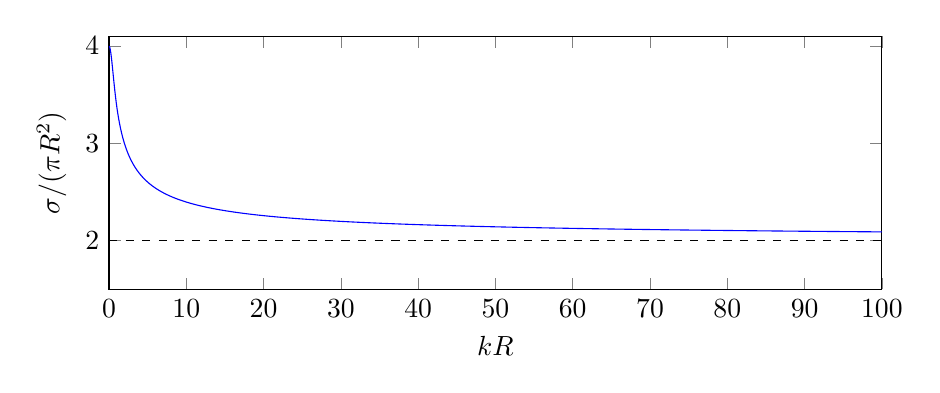
\begin{tikzpicture}\begin{axis}[width=.94\textwidth,height=4.8cm,xlabel={$kR$},ylabel={$\sigma/(\pi R^2)$},xmin=0,xmax=100,ymin=1.5,ymax=4.1]
\addplot[blue,no marks] coordinates {(0.04,3.9978705) (0.13996,3.9744496) (0.23992,3.9279674) (0.33988,3.8639153) (0.43984,3.788851) (0.5398,3.7090135) (0.63976,3.6293926) (0.73972,3.5533697) (0.83968,3.4828072) (0.93964,3.4183852) (1.0396,3.3600059) (1.1396,3.3071531) (1.2395,3.2591572) (1.3395,3.2153571) (1.4394,3.1751776) (1.5394,3.1381494) (1.6394,3.1038965) (1.7393,3.0721139) (1.8393,3.0425446) (1.9392,3.0149649) (2.0392,2.9891756) (2.1392,2.9649989) (2.2391,2.9422771) (2.3391,2.9208721) (2.439,2.9006638) (2.539,2.881548) (2.639,2.8634338) (2.7389,2.8462407) (2.8389,2.8298967) (2.9388,2.8143368) (3.0388,2.7995021) (3.1388,2.7853394) (3.2387,2.7718006) (3.3387,2.7588422) (3.4386,2.7464251) (3.5386,2.734514) (3.6386,2.7230766) (3.7385,2.7120835) (3.8385,2.7015075) (3.9384,2.6913237) (4.0384,2.6815092) (4.1384,2.6720426) (4.2383,2.6629045) (4.3383,2.6540768) (4.4382,2.6455429) (4.5382,2.6372874) (4.6382,2.629296) (4.7381,2.6215553) (4.8381,2.614053) (4.938,2.6067772) (5.038,2.5997173) (5.138,2.592863) (5.2379,2.5862048) (5.3379,2.5797339) (5.4378,2.5734419) (5.5378,2.5673209) (5.6378,2.5613637) (5.7377,2.5555632) (5.8377,2.5499129) (5.9376,2.5444067) (6.0376,2.5390386) (6.1376,2.5338032) (6.2375,2.5286953) (6.3375,2.5237099) (6.4374,2.5188424) (6.5374,2.5140883) (6.6374,2.5094435) (6.7373,2.504904) (6.8373,2.5004659) (6.9372,2.4961256) (7.0372,2.4918798) (7.1372,2.4877251) (7.2371,2.4836584) (7.3371,2.4796769) (7.437,2.4757775) (7.537,2.4719577) (7.637,2.4682149) (7.7369,2.4645465) (7.8369,2.4609503) (7.9368,2.4574239) (8.0368,2.4539652) (8.1368,2.4505722) (8.2367,2.4472428) (8.3367,2.4439751) (8.4366,2.4407674) (8.5366,2.4376179) (8.6366,2.4345248) (8.7365,2.4314866) (8.8365,2.4285018) (8.9364,2.4255687) (9.0364,2.4226861) (9.1364,2.4198525) (9.2363,2.4170666) (9.3363,2.4143271) (9.4362,2.4116327) (9.5362,2.4089824) (9.6362,2.4063749) (9.7361,2.4038091) (9.8361,2.401284) (9.936,2.3987985) (10.036,2.3963518) (10.136,2.3939426) (10.236,2.3915703) (10.336,2.3892338) (10.436,2.3869324) (10.536,2.3846651) (10.636,2.3824312) (10.736,2.3802298) (10.836,2.3780603) (10.936,2.3759218) (11.036,2.3738137) (11.136,2.3717353) (11.236,2.3696859) (11.335,2.3676649) (11.435,2.3656717) (11.535,2.3637055) (11.635,2.361766) (11.735,2.3598524) (11.835,2.3579642) (11.935,2.3561009) (12.035,2.3542619) (12.135,2.3524468) (12.235,2.3506551) (12.335,2.3488862) (12.435,2.3471397) (12.535,2.3454152) (12.635,2.3437122) (12.735,2.3420303) (12.835,2.340369) (12.935,2.338728) (13.035,2.3371069) (13.135,2.3355053) (13.235,2.3339228) (13.335,2.332359) (13.435,2.3308136) (13.535,2.3292863) (13.635,2.3277766) (13.735,2.3262844) (13.834,2.3248092) (13.934,2.3233507) (14.034,2.3219087) (14.134,2.3204829) (14.234,2.3190729) (14.334,2.3176785) (14.434,2.3162994) (14.534,2.3149353) (14.634,2.313586) (14.734,2.3122512) (14.834,2.3109307) (14.934,2.3096242) (15.034,2.3083315) (15.134,2.3070524) (15.234,2.3057865) (15.334,2.3045338) (15.434,2.303294) (15.534,2.3020668) (15.634,2.3008521) (15.734,2.2996497) (15.834,2.2984593) (15.934,2.2972809) (16.034,2.2961141) (16.134,2.2949588) (16.234,2.2938148) (16.333,2.292682) (16.433,2.2915601) (16.533,2.290449) (16.633,2.2893486) (16.733,2.2882586) (16.833,2.287179) (16.933,2.2861095) (17.033,2.2850499) (17.133,2.2840003) (17.233,2.2829604) (17.333,2.28193) (17.433,2.280909) (17.533,2.2798973) (17.633,2.2788948) (17.733,2.2779013) (17.833,2.2769167) (17.933,2.2759408) (18.033,2.2749736) (18.133,2.2740149) (18.233,2.2730645) (18.333,2.2721225) (18.433,2.2711886) (18.533,2.2702628) (18.633,2.2693449) (18.733,2.2684348) (18.832,2.2675324) (18.932,2.2666377) (19.032,2.2657505) (19.132,2.2648707) (19.232,2.2639982) (19.332,2.2631329) (19.432,2.2622747) (19.532,2.2614236) (19.632,2.2605794) (19.732,2.259742) (19.832,2.2589114) (19.932,2.2580875) (20.032,2.2572702) (20.132,2.2564593) (20.232,2.2556549) (20.332,2.2548568) (20.432,2.254065) (20.532,2.2532793) (20.632,2.2524997) (20.732,2.2517262) (20.832,2.2509586) (20.932,2.2501969) (21.032,2.249441) (21.132,2.2486908) (21.232,2.2479463) (21.331,2.2472074) (21.431,2.246474) (21.531,2.2457461) (21.631,2.2450235) (21.731,2.2443064) (21.831,2.2435944) (21.931,2.2428877) (22.031,2.2421861) (22.131,2.2414897) (22.231,2.2407982) (22.331,2.2401117) (22.431,2.2394302) (22.531,2.2387535) (22.631,2.2380815) (22.731,2.2374144) (22.831,2.2367519) (22.931,2.2360941) (23.031,2.2354409) (23.131,2.2347921) (23.231,2.2341479) (23.331,2.2335082) (23.431,2.2328728) (23.531,2.2322417) (23.631,2.231615) (23.731,2.2309925) (23.83,2.2303741) (23.93,2.22976) (24.03,2.2291499) (24.13,2.228544) (24.23,2.227942) (24.33,2.227344) (24.43,2.22675) (24.53,2.2261598) (24.63,2.2255736) (24.73,2.2249911) (24.83,2.2244124) (24.93,2.2238374) (25.03,2.2232662) (25.13,2.2226986) (25.23,2.2221346) (25.33,2.2215742) (25.43,2.2210173) (25.53,2.220464) (25.63,2.2199142) (25.73,2.2193677) (25.83,2.2188247) (25.93,2.2182851) (26.03,2.2177488) (26.13,2.2172158) (26.23,2.2166861) (26.329,2.2161596) (26.429,2.2156364) (26.529,2.2151163) (26.629,2.2145994) (26.729,2.2140856) (26.829,2.2135748) (26.929,2.2130672) (27.029,2.2125625) (27.129,2.2120609) (27.229,2.2115622) (27.329,2.2110665) (27.429,2.2105737) (27.529,2.2100838) (27.629,2.2095967) (27.729,2.2091125) (27.829,2.2086311) (27.929,2.2081525) (28.029,2.2076766) (28.129,2.2072034) (28.229,2.206733) (28.329,2.2062652) (28.429,2.2058001) (28.529,2.2053376) (28.629,2.2048778) (28.729,2.2044205) (28.828,2.2039658) (28.928,2.2035136) (29.028,2.2030639) (29.128,2.2026168) (29.228,2.2021721) (29.328,2.2017298) (29.428,2.20129) (29.528,2.2008526) (29.628,2.2004176) (29.728,2.1999849) (29.828,2.1995546) (29.928,2.1991266) (30.028,2.1987009) (30.128,2.1982775) (30.228,2.1978563) (30.328,2.1974374) (30.428,2.1970207) (30.528,2.1966063) (30.628,2.196194) (30.728,2.1957839) (30.828,2.1953759) (30.928,2.1949701) (31.028,2.1945664) (31.128,2.1941648) (31.228,2.1937652) (31.327,2.1933678) (31.427,2.1929724) (31.527,2.192579) (31.627,2.1921876) (31.727,2.1917982) (31.827,2.1914108) (31.927,2.1910253) (32.027,2.1906419) (32.127,2.1902603) (32.227,2.1898806) (32.327,2.1895029) (32.427,2.189127) (32.527,2.1887531) (32.627,2.1883809) (32.727,2.1880106) (32.827,2.1876422) (32.927,2.1872755) (33.027,2.1869107) (33.127,2.1865476) (33.227,2.1861863) (33.327,2.1858267) (33.427,2.1854689) (33.527,2.1851129) (33.627,2.1847585) (33.727,2.1844058) (33.826,2.1840549) (33.926,2.1837056) (34.026,2.183358) (34.126,2.183012) (34.226,2.1826676) (34.326,2.1823249) (34.426,2.1819838) (34.526,2.1816443) (34.626,2.1813064) (34.726,2.1809701) (34.826,2.1806353) (34.926,2.1803021) (35.026,2.1799704) (35.126,2.1796403) (35.226,2.1793117) (35.326,2.1789845) (35.426,2.1786589) (35.526,2.1783348) (35.626,2.1780121) (35.726,2.177691) (35.826,2.1773712) (35.926,2.1770529) (36.026,2.1767361) (36.126,2.1764206) (36.226,2.1761066) (36.325,2.175794) (36.425,2.1754828) (36.525,2.1751729) (36.625,2.1748644) (36.725,2.1745573) (36.825,2.1742516) (36.925,2.1739472) (37.025,2.1736441) (37.125,2.1733423) (37.225,2.1730419) (37.325,2.1727427) (37.425,2.1724449) (37.525,2.1721484) (37.625,2.1718531) (37.725,2.1715591) (37.825,2.1712664) (37.925,2.1709749) (38.025,2.1706846) (38.125,2.1703956) (38.225,2.1701079) (38.325,2.1698213) (38.425,2.169536) (38.525,2.1692518) (38.625,2.1689689) (38.725,2.1686871) (38.824,2.1684066) (38.924,2.1681271) (39.024,2.1678489) (39.124,2.1675718) (39.224,2.1672959) (39.324,2.1670211) (39.424,2.1667474) (39.524,2.1664748) (39.624,2.1662034) (39.724,2.1659331) (39.824,2.1656639) (39.924,2.1653958) (40.024,2.1651287) (40.124,2.1648628) (40.224,2.1645979) (40.324,2.1643341) (40.424,2.1640713) (40.524,2.1638097) (40.624,2.163549) (40.724,2.1632894) (40.824,2.1630308) (40.924,2.1627733) (41.024,2.1625168) (41.124,2.1622613) (41.224,2.1620068) (41.323,2.1617533) (41.423,2.1615007) (41.523,2.1612492) (41.623,2.1609987) (41.723,2.1607491) (41.823,2.1605006) (41.923,2.1602529) (42.023,2.1600063) (42.123,2.1597606) (42.223,2.1595158) (42.323,2.159272) (42.423,2.1590291) (42.523,2.1587871) (42.623,2.1585461) (42.723,2.158306) (42.823,2.1580667) (42.923,2.1578284) (43.023,2.157591) (43.123,2.1573545) (43.223,2.1571189) (43.323,2.1568842) (43.423,2.1566503) (43.523,2.1564174) (43.623,2.1561853) (43.723,2.155954) (43.822,2.1557236) (43.922,2.1554941) (44.022,2.1552654) (44.122,2.1550376) (44.222,2.1548106) (44.322,2.1545844) (44.422,2.1543591) (44.522,2.1541346) (44.622,2.1539109) (44.722,2.153688) (44.822,2.1534659) (44.922,2.1532447) (45.022,2.1530242) (45.122,2.1528045) (45.222,2.1525857) (45.322,2.1523676) (45.422,2.1521503) (45.522,2.1519337) (45.622,2.151718) (45.722,2.151503) (45.822,2.1512888) (45.922,2.1510753) (46.022,2.1508626) (46.122,2.1506506) (46.222,2.1504394) (46.321,2.1502289) (46.421,2.1500192) (46.521,2.1498102) (46.621,2.1496019) (46.721,2.1493944) (46.821,2.1491876) (46.921,2.1489815) (47.021,2.1487761) (47.121,2.1485714) (47.221,2.1483674) (47.321,2.1481642) (47.421,2.1479616) (47.521,2.1477597) (47.621,2.1475586) (47.721,2.1473581) (47.821,2.1471582) (47.921,2.1469591) (48.021,2.1467606) (48.121,2.1465629) (48.221,2.1463657) (48.321,2.1461693) (48.421,2.1459735) (48.521,2.1457784) (48.621,2.1455839) (48.721,2.1453901) (48.82,2.1451969) (48.92,2.1450043) (49.02,2.1448124) (49.12,2.1446212) (49.22,2.1444306) (49.32,2.1442406) (49.42,2.1440512) (49.52,2.1438624) (49.62,2.1436743) (49.72,2.1434868) (49.82,2.1432999) (49.92,2.1431136) (50.02,2.1429279) (50.12,2.1427429) (50.22,2.1425584) (50.32,2.1423745) (50.42,2.1421912) (50.52,2.1420086) (50.62,2.1418265) (50.72,2.1416449) (50.82,2.141464) (50.92,2.1412837) (51.02,2.1411039) (51.12,2.1409247) (51.22,2.1407461) (51.319,2.140568) (51.419,2.1403905) (51.519,2.1402136) (51.619,2.1400372) (51.719,2.1398614) (51.819,2.1396861) (51.919,2.1395114) (52.019,2.1393372) (52.119,2.1391636) (52.219,2.1389905) (52.319,2.138818) (52.419,2.138646) (52.519,2.1384745) (52.619,2.1383036) (52.719,2.1381332) (52.819,2.1379633) (52.919,2.1377939) (53.019,2.1376251) (53.119,2.1374568) (53.219,2.137289) (53.319,2.1371217) (53.419,2.1369549) (53.519,2.1367886) (53.619,2.1366229) (53.719,2.1364576) (53.818,2.1362929) (53.918,2.1361286) (54.018,2.1359648) (54.118,2.1358016) (54.218,2.1356388) (54.318,2.1354765) (54.418,2.1353147) (54.518,2.1351534) (54.618,2.1349926) (54.718,2.1348322) (54.818,2.1346723) (54.918,2.1345129) (55.018,2.134354) (55.118,2.1341956) (55.218,2.1340376) (55.318,2.13388) (55.418,2.133723) (55.518,2.1335664) (55.618,2.1334103) (55.718,2.1332546) (55.818,2.1330994) (55.918,2.1329446) (56.018,2.1327903) (56.118,2.1326364) (56.218,2.132483) (56.317,2.13233) (56.417,2.1321775) (56.517,2.1320254) (56.617,2.1318737) (56.717,2.1317225) (56.817,2.1315717) (56.917,2.1314214) (57.017,2.1312715) (57.117,2.131122) (57.217,2.1309729) (57.317,2.1308243) (57.417,2.1306761) (57.517,2.1305283) (57.617,2.1303809) (57.717,2.1302339) (57.817,2.1300874) (57.917,2.1299413) (58.017,2.1297956) (58.117,2.1296503) (58.217,2.1295054) (58.317,2.1293609) (58.417,2.1292168) (58.517,2.1290731) (58.617,2.1289298) (58.717,2.1287869) (58.816,2.1286444) (58.916,2.1285023) (59.016,2.1283606) (59.116,2.1282193) (59.216,2.1280784) (59.316,2.1279379) (59.416,2.1277977) (59.516,2.127658) (59.616,2.1275186) (59.716,2.1273796) (59.816,2.127241) (59.916,2.1271028) (60.016,2.1269649) (60.116,2.1268274) (60.216,2.1266903) (60.316,2.1265536) (60.416,2.1264172) (60.516,2.1262812) (60.616,2.1261455) (60.716,2.1260103) (60.816,2.1258754) (60.916,2.1257408) (61.016,2.1256066) (61.116,2.1254728) (61.216,2.1253394) (61.315,2.1252062) (61.415,2.1250735) (61.515,2.1249411) (61.615,2.124809) (61.715,2.1246773) (61.815,2.124546) (61.915,2.124415) (62.015,2.1242843) (62.115,2.124154) (62.215,2.124024) (62.315,2.1238944) (62.415,2.1237651) (62.515,2.1236361) (62.615,2.1235075) (62.715,2.1233792) (62.815,2.1232513) (62.915,2.1231237) (63.015,2.1229964) (63.115,2.1228694) (63.215,2.1227428) (63.315,2.1226165) (63.415,2.1224905) (63.515,2.1223649) (63.615,2.1222396) (63.715,2.1221146) (63.814,2.1219899) (63.914,2.1218655) (64.014,2.1217415) (64.114,2.1216177) (64.214,2.1214943) (64.314,2.1213712) (64.414,2.1212484) (64.514,2.121126) (64.614,2.1210038) (64.714,2.1208819) (64.814,2.1207604) (64.914,2.1206391) (65.014,2.1205182) (65.114,2.1203976) (65.214,2.1202772) (65.314,2.1201572) (65.414,2.1200375) (65.514,2.119918) (65.614,2.1197989) (65.714,2.1196801) (65.814,2.1195615) (65.914,2.1194433) (66.014,2.1193253) (66.114,2.1192077) (66.214,2.1190903) (66.313,2.1189732) (66.413,2.1188564) (66.513,2.1187399) (66.613,2.1186237) (66.713,2.1185078) (66.813,2.1183921) (66.913,2.1182768) (67.013,2.1181617) (67.113,2.1180469) (67.213,2.1179324) (67.313,2.1178181) (67.413,2.1177041) (67.513,2.1175904) (67.613,2.117477) (67.713,2.1173639) (67.813,2.117251) (67.913,2.1171384) (68.013,2.1170261) (68.113,2.116914) (68.213,2.1168023) (68.313,2.1166907) (68.413,2.1165795) (68.513,2.1164685) (68.613,2.1163578) (68.713,2.1162473) (68.812,2.1161371) (68.912,2.1160272) (69.012,2.1159175) (69.112,2.1158081) (69.212,2.115699) (69.312,2.1155901) (69.412,2.1154814) (69.512,2.115373) (69.612,2.1152649) (69.712,2.115157) (69.812,2.1150494) (69.912,2.1149421) (70.012,2.1148349) (70.112,2.1147281) (70.212,2.1146215) (70.312,2.1145151) (70.412,2.114409) (70.512,2.1143031) (70.612,2.1141975) (70.712,2.1140921) (70.812,2.1139869) (70.912,2.113882) (71.012,2.1137774) (71.112,2.113673) (71.212,2.1135688) (71.311,2.1134649) (71.411,2.1133612) (71.511,2.1132577) (71.611,2.1131545) (71.711,2.1130515) (71.811,2.1129487) (71.911,2.1128462) (72.011,2.1127439) (72.111,2.1126419) (72.211,2.1125401) (72.311,2.1124385) (72.411,2.1123371) (72.511,2.112236) (72.611,2.1121351) (72.711,2.1120344) (72.811,2.111934) (72.911,2.1118337) (73.011,2.1117337) (73.111,2.111634) (73.211,2.1115344) (73.311,2.1114351) (73.411,2.111336) (73.511,2.1112371) (73.611,2.1111384) (73.711,2.11104) (73.81,2.1109418) (73.91,2.1108438) (74.01,2.110746) (74.11,2.1106484) (74.21,2.110551) (74.31,2.1104539) (74.41,2.1103569) (74.51,2.1102602) (74.61,2.1101637) (74.71,2.1100674) (74.81,2.1099713) (74.91,2.1098755) (75.01,2.1097798) (75.11,2.1096844) (75.21,2.1095891) (75.31,2.1094941) (75.41,2.1093992) (75.51,2.1093046) (75.61,2.1092102) (75.71,2.109116) (75.81,2.109022) (75.91,2.1089281) (76.01,2.1088345) (76.11,2.1087411) (76.21,2.1086479) (76.309,2.1085549) (76.409,2.1084621) (76.509,2.1083695) (76.609,2.1082771) (76.709,2.1081849) (76.809,2.1080929) (76.909,2.1080011) (77.009,2.1079094) (77.109,2.107818) (77.209,2.1077268) (77.309,2.1076357) (77.409,2.1075449) (77.509,2.1074542) (77.609,2.1073638) (77.709,2.1072735) (77.809,2.1071834) (77.909,2.1070935) (78.009,2.1070038) (78.109,2.1069143) (78.209,2.106825) (78.309,2.1067358) (78.409,2.1066469) (78.509,2.1065581) (78.609,2.1064695) (78.709,2.1063811) (78.808,2.1062929) (78.908,2.1062049) (79.008,2.106117) (79.108,2.1060294) (79.208,2.1059419) (79.308,2.1058546) (79.408,2.1057674) (79.508,2.1056805) (79.608,2.1055937) (79.708,2.1055071) (79.808,2.1054207) (79.908,2.1053345) (80.008,2.1052484) (80.108,2.1051626) (80.208,2.1050769) (80.308,2.1049913) (80.408,2.104906) (80.508,2.1048208) (80.608,2.1047358) (80.708,2.104651) (80.808,2.1045663) (80.908,2.1044818) (81.008,2.1043975) (81.108,2.1043134) (81.208,2.1042294) (81.307,2.1041456) (81.407,2.1040619) (81.507,2.1039785) (81.607,2.1038952) (81.707,2.103812) (81.807,2.103729) (81.907,2.1036462) (82.007,2.1035636) (82.107,2.1034811) (82.207,2.1033988) (82.307,2.1033167) (82.407,2.1032347) (82.507,2.1031529) (82.607,2.1030712) (82.707,2.1029897) (82.807,2.1029084) (82.907,2.1028272) (83.007,2.1027462) (83.107,2.1026654) (83.207,2.1025847) (83.307,2.1025042) (83.407,2.1024238) (83.507,2.1023436) (83.607,2.1022635) (83.707,2.1021836) (83.806,2.1021039) (83.906,2.1020243) (84.006,2.1019449) (84.106,2.1018656) (84.206,2.1017865) (84.306,2.1017075) (84.406,2.1016287) (84.506,2.10155) (84.606,2.1014715) (84.706,2.1013931) (84.806,2.1013149) (84.906,2.1012369) (85.006,2.101159) (85.106,2.1010812) (85.206,2.1010036) (85.306,2.1009262) (85.406,2.1008489) (85.506,2.1007717) (85.606,2.1006947) (85.706,2.1006178) (85.806,2.1005411) (85.906,2.1004645) (86.006,2.1003881) (86.106,2.1003118) (86.206,2.1002357) (86.305,2.1001597) (86.405,2.1000839) (86.505,2.1000082) (86.605,2.0999326) (86.705,2.0998572) (86.805,2.0997819) (86.905,2.0997068) (87.005,2.0996318) (87.105,2.099557) (87.205,2.0994823) (87.305,2.0994077) (87.405,2.0993333) (87.505,2.099259) (87.605,2.0991849) (87.705,2.0991109) (87.805,2.099037) (87.905,2.0989633) (88.005,2.0988897) (88.105,2.0988162) (88.205,2.0987429) (88.305,2.0986697) (88.405,2.0985967) (88.505,2.0985238) (88.605,2.098451) (88.705,2.0983784) (88.804,2.0983059) (88.904,2.0982335) (89.004,2.0981613) (89.104,2.0980892) (89.204,2.0980172) (89.304,2.0979453) (89.404,2.0978736) (89.504,2.0978021) (89.604,2.0977306) (89.704,2.0976593) (89.804,2.0975881) (89.904,2.0975171) (90.004,2.0974461) (90.104,2.0973753) (90.204,2.0973047) (90.304,2.0972341) (90.404,2.0971637) (90.504,2.0970934) (90.604,2.0970233) (90.704,2.0969533) (90.804,2.0968834) (90.904,2.0968136) (91.004,2.0967439) (91.104,2.0966744) (91.204,2.096605) (91.303,2.0965358) (91.403,2.0964666) (91.503,2.0963976) (91.603,2.0963287) (91.703,2.0962599) (91.803,2.0961913) (91.903,2.0961227) (92.003,2.0960543) (92.103,2.095986) (92.203,2.0959179) (92.303,2.0958498) (92.403,2.0957819) (92.503,2.0957141) (92.603,2.0956464) (92.703,2.0955788) (92.803,2.0955114) (92.903,2.0954441) (93.003,2.0953769) (93.103,2.0953098) (93.203,2.0952428) (93.303,2.095176) (93.403,2.0951092) (93.503,2.0950426) (93.603,2.0949761) (93.703,2.0949098) (93.802,2.0948435) (93.902,2.0947773) (94.002,2.0947113) (94.102,2.0946454) (94.202,2.0945796) (94.302,2.0945139) (94.402,2.0944483) (94.502,2.0943829) (94.602,2.0943175) (94.702,2.0942523) (94.802,2.0941872) (94.902,2.0941222) (95.002,2.0940573) (95.102,2.0939925) (95.202,2.0939278) (95.302,2.0938633) (95.402,2.0937988) (95.502,2.0937345) (95.602,2.0936702) (95.702,2.0936061) (95.802,2.0935421) (95.902,2.0934782) (96.002,2.0934144) (96.102,2.0933508) (96.202,2.0932872) (96.301,2.0932237) (96.401,2.0931604) (96.501,2.0930971) (96.601,2.093034) (96.701,2.092971) (96.801,2.092908) (96.901,2.0928452) (97.001,2.0927825) (97.101,2.0927199) (97.201,2.0926574) (97.301,2.092595) (97.401,2.0925327) (97.501,2.0924705) (97.601,2.0924085) (97.701,2.0923465) (97.801,2.0922846) (97.901,2.0922229) (98.001,2.0921612) (98.101,2.0920996) (98.201,2.0920382) (98.301,2.0919768) (98.401,2.0919156) (98.501,2.0918544) (98.601,2.0917934) (98.701,2.0917325) (98.8,2.0916716) (98.9,2.0916109) (99,2.0915502) (99.1,2.0914897) (99.2,2.0914292) (99.3,2.0913689) (99.4,2.0913087) (99.5,2.0912485) (99.6,2.0911885) (99.7,2.0911285) (99.8,2.0910687) (99.9,2.091009) (100,2.0909493)};
\addplot[dashed] coordinates {(0,2)(100,2)};
\end{axis}\end{tikzpicture}\caption{硬球总截面从低能$4\pi R^2$趋向高能$2\pi R^2$，横轴完整覆盖至100。}\end{figure}
\begin{figure}[htbp]\centering\begin{tikzpicture}\begin{axis}[width=.94\textwidth,height=4.8cm,xlabel={$\theta$（度）},ylabel={$(\dd\sigma/\dd\Omega)/(Z^2a_0^2)$},xmin=0,xmax=180]
\addplot[blue,no marks] coordinates {(0.000,0.04) (0.300,0.039994243) (0.600,0.039976978) (0.900,0.039948221) (1.200,0.039907997) (1.500,0.039856343) (1.800,0.039793305) (2.100,0.039718941) (2.400,0.039633318) (2.700,0.039536513) (3.000,0.039428613) (3.300,0.039309715) (3.600,0.039179925) (3.900,0.03903936) (4.200,0.038888145) (4.500,0.038726415) (4.800,0.038554313) (5.100,0.03837199) (5.400,0.038179608) (5.700,0.037977336) (6.000,0.03776535) (6.300,0.037543835) (6.600,0.037312983) (6.900,0.037072992) (7.200,0.03682407) (7.500,0.036566429) (7.800,0.036300287) (8.100,0.036025869) (8.400,0.035743406) (8.700,0.035453134) (9.000,0.035155294) (9.300,0.03485013) (9.600,0.034537893) (9.900,0.034218836) (10.200,0.033893217) (10.500,0.033561295) (10.800,0.033223334) (11.100,0.032879601) (11.400,0.032530363) (11.700,0.03217589) (12.000,0.031816454) (12.300,0.031452327) (12.600,0.031083783) (12.900,0.030711095) (13.200,0.030334538) (13.500,0.029954385) (13.800,0.029570909) (14.100,0.029184383) (14.400,0.028795078) (14.700,0.028403263) (15.000,0.028009207) (15.300,0.027613175) (15.600,0.02721543) (15.900,0.026816232) (16.200,0.026415841) (16.500,0.026014509) (16.800,0.025612489) (17.100,0.025210026) (17.400,0.024807366) (17.700,0.024404746) (18.000,0.024002401) (18.300,0.023600562) (18.600,0.023199454) (18.900,0.022799298) (19.200,0.022400308) (19.500,0.022002694) (19.800,0.021606662) (20.100,0.021212409) (20.400,0.020820129) (20.700,0.02043001) (21.000,0.020042233) (21.300,0.019656972) (21.600,0.019274399) (21.900,0.018894674) (22.200,0.018517957) (22.500,0.018144396) (22.800,0.017774136) (23.100,0.017407316) (23.400,0.017044066) (23.700,0.016684512) (24.000,0.016328773) (24.300,0.015976961) (24.600,0.015629182) (24.900,0.015285536) (25.200,0.014946118) (25.500,0.014611013) (25.800,0.014280303) (26.100,0.013954065) (26.400,0.013632365) (26.700,0.013315269) (27.000,0.013002833) (27.300,0.012695109) (27.600,0.012392143) (27.900,0.012093975) (28.200,0.01180064) (28.500,0.011512169) (28.800,0.011228585) (29.100,0.010949908) (29.400,0.010676153) (29.700,0.010407329) (30.000,0.010143441) (30.300,0.0098844905) (30.600,0.0096304726) (30.900,0.0093813795) (31.200,0.0091371992) (31.500,0.0088979153) (31.800,0.008663508) (32.100,0.0084339537) (32.400,0.0082092253) (32.700,0.0079892924) (33.000,0.0077741213) (33.300,0.0075636753) (33.600,0.007357915) (33.900,0.0071567979) (34.200,0.0069602792) (34.500,0.0067683115) (34.800,0.0065808452) (35.100,0.0063978283) (35.400,0.0062192072) (35.700,0.0060449259) (36.000,0.0058749271) (36.300,0.0057091517) (36.600,0.0055475392) (36.900,0.0053900275) (37.200,0.0052365536) (37.500,0.0050870534) (37.800,0.0049414615) (38.100,0.0047997119) (38.400,0.0046617378) (38.700,0.0045274718) (39.000,0.0043968459) (39.300,0.0042697917) (39.600,0.0041462404) (39.900,0.0040261232) (40.200,0.0039093708) (40.500,0.0037959142) (40.800,0.0036856842) (41.100,0.0035786119) (41.400,0.0034746284) (41.700,0.0033736651) (42.000,0.0032756539) (42.300,0.0031805269) (42.600,0.0030882168) (42.900,0.0029986567) (43.200,0.0029117805) (43.500,0.0028275224) (43.800,0.0027458175) (44.100,0.0026666017) (44.400,0.0025898115) (44.700,0.0025153842) (45.000,0.002443258) (45.300,0.002373372) (45.600,0.0023056662) (45.900,0.0022400815) (46.200,0.0021765598) (46.500,0.0021150439) (46.800,0.0020554776) (47.100,0.0019978058) (47.400,0.0019419744) (47.700,0.0018879303) (48.000,0.0018356216) (48.300,0.0017849971) (48.600,0.001736007) (48.900,0.0016886026) (49.200,0.0016427359) (49.500,0.0015983603) (49.800,0.0015554303) (50.100,0.0015139011) (50.400,0.0014737293) (50.700,0.0014348724) (51.000,0.0013972891) (51.300,0.0013609389) (51.600,0.0013257826) (51.900,0.0012917818) (52.200,0.0012588991) (52.500,0.0012270983) (52.800,0.001196344) (53.100,0.0011666019) (53.400,0.0011378386) (53.700,0.0011100214) (54.000,0.0010831191) (54.300,0.0010571007) (54.600,0.0010319367) (54.900,0.0010075981) (55.200,0.00098405691) (55.500,0.00096128594) (55.800,0.00093925881) (56.100,0.00091794997) (56.400,0.00089733466) (56.700,0.00087738885) (57.000,0.0008580893) (57.300,0.00083941349) (57.600,0.00082133961) (57.900,0.00080384655) (58.200,0.00078691387) (58.500,0.00077052182) (58.800,0.00075465126) (59.100,0.0007392837) (59.400,0.00072440125) (59.700,0.00070998663) (60.000,0.0006960231) (60.300,0.00068249452) (60.600,0.00066938528) (60.900,0.0006566803) (61.200,0.000644365) (61.500,0.00063242532) (61.800,0.00062084767) (62.100,0.00060961892) (62.400,0.00059872643) (62.700,0.00058815796) (63.000,0.00057790171) (63.300,0.00056794631) (63.600,0.00055828077) (63.900,0.0005488945) (64.200,0.00053977728) (64.500,0.00053091926) (64.800,0.00052231093) (65.100,0.00051394313) (65.400,0.00050580704) (65.700,0.00049789413) (66.000,0.00049019621) (66.300,0.00048270536) (66.600,0.00047541398) (66.900,0.00046831472) (67.200,0.00046140051) (67.500,0.00045466455) (67.800,0.00044810029) (68.100,0.00044170141) (68.400,0.00043546183) (68.700,0.00042937572) (69.000,0.00042343743) (69.300,0.00041764156) (69.600,0.0004119829) (69.900,0.00040645644) (70.200,0.00040105735) (70.500,0.000395781) (70.800,0.00039062294) (71.100,0.00038557888) (71.400,0.00038064471) (71.700,0.00037581647) (72.000,0.00037109036) (72.300,0.00036646274) (72.600,0.00036193011) (72.900,0.00035748908) (73.200,0.00035313644) (73.500,0.0003488691) (73.800,0.00034468406) (74.100,0.00034057849) (74.400,0.00033654964) (74.700,0.00033259489) (75.000,0.00032871174) (75.300,0.00032489777) (75.600,0.00032115066) (75.900,0.00031746822) (76.200,0.00031384833) (76.500,0.00031028895) (76.800,0.00030678815) (77.100,0.00030334407) (77.400,0.00029995493) (77.700,0.00029661905) (78.000,0.00029333478) (78.300,0.00029010059) (78.600,0.00028691499) (78.900,0.00028377656) (79.200,0.00028068395) (79.500,0.00027763586) (79.800,0.00027463107) (80.100,0.0002716684) (80.400,0.00026874671) (80.700,0.00026586495) (81.000,0.00026302208) (81.300,0.00026021714) (81.600,0.00025744919) (81.900,0.00025471735) (82.200,0.00025202077) (82.500,0.00024935866) (82.800,0.00024673023) (83.100,0.00024413477) (83.400,0.00024157157) (83.700,0.00023903997) (84.000,0.00023653935) (84.300,0.00023406909) (84.600,0.00023162863) (84.900,0.00022921742) (85.200,0.00022683494) (85.500,0.0002244807) (85.800,0.00022215421) (86.100,0.00021985503) (86.400,0.00021758273) (86.700,0.0002153369) (87.000,0.00021311714) (87.300,0.00021092309) (87.600,0.00020875438) (87.900,0.00020661066) (88.200,0.00020449163) (88.500,0.00020239695) (88.800,0.00020032633) (89.100,0.00019827948) (89.400,0.00019625613) (89.700,0.000194256) (90.000,0.00019227884) (90.300,0.0001903244) (90.600,0.00018839245) (90.900,0.00018648275) (91.200,0.00018459509) (91.500,0.00018272923) (91.800,0.00018088499) (92.100,0.00017906214) (92.400,0.0001772605) (92.700,0.00017547987) (93.000,0.00017372006) (93.300,0.0001719809) (93.600,0.00017026218) (93.900,0.00016856375) (94.200,0.00016688543) (94.500,0.00016522704) (94.800,0.00016358843) (95.100,0.00016196941) (95.400,0.00016036983) (95.700,0.00015878953) (96.000,0.00015722835) (96.300,0.00015568612) (96.600,0.00015416269) (96.900,0.00015265791) (97.200,0.00015117161) (97.500,0.00014970364) (97.800,0.00014825386) (98.100,0.00014682209) (98.400,0.0001454082) (98.700,0.00014401202) (99.000,0.00014263341) (99.300,0.00014127221) (99.600,0.00013992827) (99.900,0.00013860144) (100.200,0.00013729156) (100.500,0.00013599848) (100.800,0.00013472204) (101.100,0.00013346211) (101.400,0.00013221851) (101.700,0.00013099111) (102.000,0.00012977973) (102.300,0.00012858425) (102.600,0.00012740448) (102.900,0.0001262403) (103.200,0.00012509153) (103.500,0.00012395803) (103.800,0.00012283964) (104.100,0.0001217362) (104.400,0.00012064757) (104.700,0.00011957358) (105.000,0.00011851409) (105.300,0.00011746893) (105.600,0.00011643796) (105.900,0.00011542102) (106.200,0.00011441795) (106.500,0.0001134286) (106.800,0.00011245282) (107.100,0.00011149045) (107.400,0.00011054133) (107.700,0.00010960533) (108.000,0.00010868227) (108.300,0.00010777201) (108.600,0.0001068744) (108.900,0.00010598928) (109.200,0.00010511651) (109.500,0.00010425593) (109.800,0.00010340739) (110.100,0.00010257074) (110.400,0.00010174584) (110.700,0.00010093253) (111.000,0.00010013067) (111.300,9.9340106e-05) (111.600,9.8560701e-05) (111.900,9.7792305e-05) (112.200,9.7034774e-05) (112.500,9.6287965e-05) (112.800,9.5551734e-05) (113.100,9.4825941e-05) (113.400,9.4110445e-05) (113.700,9.3405106e-05) (114.000,9.2709785e-05) (114.300,9.2024346e-05) (114.600,9.1348651e-05) (114.900,9.0682566e-05) (115.200,9.0025956e-05) (115.500,8.9378688e-05) (115.800,8.8740631e-05) (116.100,8.8111654e-05) (116.400,8.7491627e-05) (116.700,8.6880423e-05) (117.000,8.6277914e-05) (117.300,8.5683976e-05) (117.600,8.5098483e-05) (117.900,8.4521312e-05) (118.200,8.3952343e-05) (118.500,8.3391454e-05) (118.800,8.2838526e-05) (119.100,8.2293442e-05) (119.400,8.1756086e-05) (119.700,8.1226342e-05) (120.000,8.0704096e-05) (120.300,8.0189237e-05) (120.600,7.9681654e-05) (120.900,7.9181237e-05) (121.200,7.8687877e-05) (121.500,7.8201468e-05) (121.800,7.7721905e-05) (122.100,7.7249084e-05) (122.400,7.6782902e-05) (122.700,7.6323257e-05) (123.000,7.587005e-05) (123.300,7.5423182e-05) (123.600,7.4982557e-05) (123.900,7.4548078e-05) (124.200,7.4119651e-05) (124.500,7.3697183e-05) (124.800,7.3280582e-05) (125.100,7.2869758e-05) (125.400,7.2464623e-05) (125.700,7.2065087e-05) (126.000,7.1671065e-05) (126.300,7.1282472e-05) (126.600,7.0899224e-05) (126.900,7.0521239e-05) (127.200,7.0148435e-05) (127.500,6.9780733e-05) (127.800,6.9418053e-05) (128.100,6.906032e-05) (128.400,6.8707456e-05) (128.700,6.8359388e-05) (129.000,6.801604e-05) (129.300,6.7677341e-05) (129.600,6.734322e-05) (129.900,6.7013606e-05) (130.200,6.6688431e-05) (130.500,6.6367627e-05) (130.800,6.6051128e-05) (131.100,6.5738868e-05) (131.400,6.5430782e-05) (131.700,6.5126809e-05) (132.000,6.4826886e-05) (132.300,6.4530952e-05) (132.600,6.4238946e-05) (132.900,6.3950812e-05) (133.200,6.3666489e-05) (133.500,6.3385923e-05) (133.800,6.3109057e-05) (134.100,6.2835836e-05) (134.400,6.2566208e-05) (134.700,6.2300119e-05) (135.000,6.2037517e-05) (135.300,6.1778352e-05) (135.600,6.1522574e-05) (135.900,6.1270135e-05) (136.200,6.1020985e-05) (136.500,6.0775079e-05) (136.800,6.0532369e-05) (137.100,6.0292811e-05) (137.400,6.005636e-05) (137.700,5.9822973e-05) (138.000,5.9592607e-05) (138.300,5.936522e-05) (138.600,5.9140771e-05) (138.900,5.8919219e-05) (139.200,5.8700525e-05) (139.500,5.848465e-05) (139.800,5.8271557e-05) (140.100,5.8061207e-05) (140.400,5.7853565e-05) (140.700,5.7648595e-05) (141.000,5.7446261e-05) (141.300,5.7246529e-05) (141.600,5.7049366e-05) (141.900,5.6854738e-05) (142.200,5.6662613e-05) (142.500,5.647296e-05) (142.800,5.6285746e-05) (143.100,5.6100942e-05) (143.400,5.5918519e-05) (143.700,5.5738445e-05) (144.000,5.5560694e-05) (144.300,5.5385237e-05) (144.600,5.5212046e-05) (144.900,5.5041095e-05) (145.200,5.4872357e-05) (145.500,5.4705806e-05) (145.800,5.4541417e-05) (146.100,5.4379166e-05) (146.400,5.4219027e-05) (146.700,5.4060978e-05) (147.000,5.3904994e-05) (147.300,5.3751054e-05) (147.600,5.3599134e-05) (147.900,5.3449214e-05) (148.200,5.3301271e-05) (148.500,5.3155284e-05) (148.800,5.3011234e-05) (149.100,5.28691e-05) (149.400,5.2728862e-05) (149.700,5.2590501e-05) (150.000,5.2453999e-05) (150.300,5.2319336e-05) (150.600,5.2186496e-05) (150.900,5.2055459e-05) (151.200,5.192621e-05) (151.500,5.179873e-05) (151.800,5.1673004e-05) (152.100,5.1549015e-05) (152.400,5.1426747e-05) (152.700,5.1306185e-05) (153.000,5.1187314e-05) (153.300,5.1070118e-05) (153.600,5.0954584e-05) (153.900,5.0840696e-05) (154.200,5.0728442e-05) (154.500,5.0617807e-05) (154.800,5.0508779e-05) (155.100,5.0401343e-05) (155.400,5.0295488e-05) (155.700,5.0191201e-05) (156.000,5.008847e-05) (156.300,4.9987282e-05) (156.600,4.9887627e-05) (156.900,4.9789492e-05) (157.200,4.9692867e-05) (157.500,4.959774e-05) (157.800,4.9504101e-05) (158.100,4.941194e-05) (158.400,4.9321247e-05) (158.700,4.9232011e-05) (159.000,4.9144222e-05) (159.300,4.9057872e-05) (159.600,4.8972951e-05) (159.900,4.8889449e-05) (160.200,4.8807359e-05) (160.500,4.8726671e-05) (160.800,4.8647376e-05) (161.100,4.8569467e-05) (161.400,4.8492936e-05) (161.700,4.8417774e-05) (162.000,4.8343974e-05) (162.300,4.8271528e-05) (162.600,4.820043e-05) (162.900,4.8130671e-05) (163.200,4.8062245e-05) (163.500,4.7995145e-05) (163.800,4.7929365e-05) (164.100,4.7864897e-05) (164.400,4.7801736e-05) (164.700,4.7739876e-05) (165.000,4.767931e-05) (165.300,4.7620033e-05) (165.600,4.7562038e-05) (165.900,4.7505321e-05) (166.200,4.7449877e-05) (166.500,4.7395698e-05) (166.800,4.7342782e-05) (167.100,4.7291122e-05) (167.400,4.7240714e-05) (167.700,4.7191553e-05) (168.000,4.7143635e-05) (168.300,4.7096955e-05) (168.600,4.7051508e-05) (168.900,4.7007292e-05) (169.200,4.6964301e-05) (169.500,4.6922532e-05) (169.800,4.6881982e-05) (170.100,4.6842645e-05) (170.400,4.6804519e-05) (170.700,4.6767601e-05) (171.000,4.6731887e-05) (171.300,4.6697374e-05) (171.600,4.6664059e-05) (171.900,4.6631938e-05) (172.200,4.660101e-05) (172.500,4.6571271e-05) (172.800,4.6542719e-05) (173.100,4.6515351e-05) (173.400,4.6489165e-05) (173.700,4.6464159e-05) (174.000,4.644033e-05) (174.300,4.6417676e-05) (174.600,4.6396196e-05) (174.900,4.6375887e-05) (175.200,4.6356748e-05) (175.500,4.6338777e-05) (175.800,4.6321973e-05) (176.100,4.6306334e-05) (176.400,4.6291859e-05) (176.700,4.6278546e-05) (177.000,4.6266395e-05) (177.300,4.6255404e-05) (177.600,4.6245572e-05) (177.900,4.6236899e-05) (178.200,4.6229384e-05) (178.500,4.6223027e-05) (178.800,4.6217826e-05) (179.100,4.6213781e-05) (179.400,4.6210892e-05) (179.700,4.6209159e-05) (180.000,4.6208581e-05)};
\end{axis}\end{tikzpicture}\caption{PS11 Q5：1 keV电子与均匀电子云中性原子的Born微分截面，核电荷数$Z$按比例因子保留。}\end{figure}

\end{solution}

\originalsection{PS11 Q4：指数井的精确s波}
\begin{exercise}
$V(r)=-V_0e^{-r/a}$、$V_0>0$，求$\delta_0(E)$并分析它与$l=0$束缚谱的联系。
\end{exercise}
\begin{solution}
径向$u''+[k^2+(2mV_0/\hbar^2)e^{-r/a}]u=0$。置$y=y_0e^{-r/(2a)}$、$y_0=2a\sqrt{2mV_0}/\hbar$，变成$y^2u_{yy}+yu_y+(y^2-\nu^2)u=0$、$\nu=2iak$。正能解取
\[
 u=J_{-\nu}(y_0)J_\nu(y)-J_\nu(y_0)J_{-\nu}(y),
\]
满足$u(0)=0$。大$r$用$J_\nu(y)\sim(y/2)^\nu/\Gamma(1+\nu)$读入/出射比，得
\[
 e^{2i\delta_0(k)}=\frac{J_\nu(y_0)}{J_{-\nu}(y_0)}
 (y_0/2)^{-2\nu}\frac{\Gamma(1+\nu)}{\Gamma(1-\nu)}.
\]
实$k$分子分母互为共轭，模为1；$V_0\to0$各因子相消给$S=1$。相位从高能$\delta\to0$连续展开，不把主值$\arg/2$的跳跃当共振。

束缚$E=-\hbar^2\kappa^2/(2m)$取$\nu_b=2a\kappa>0$，无穷衰减解是$J_{\nu_b}(y)$，量子化为$J_{\nu_b}(y_0)=0$；这给全部$s$波束缚能，不能用$J_\nu(y_0)$关于$y_0$的固定阶零点直接当能量。零能正则解为$J_0(y_0)Y_0(y)-Y_0(y_0)J_0(y)$，读$u\propto r-a_s$得
\[
 a_s=2a[\ln(y_0/2)+\gamma_E]-\pi a\frac{Y_0(y_0)}{J_0(y_0)}.
\]
每当$J_0(y_0)=0$，零能束缚态进入，散射长度发散；临近正大$a_s$给浅束缚能$-\hbar^2/(2ma_s^2)$。第一阈值$y_0\simeq2.4048$。无恰好零能半束缚时Levinson关系$\delta_0(0)-\delta_0(\infty)=N_0\pi$联系束缚数；阈值态需半整数修正。这里引用该短程谱定理作为进阶输入，没有将上述局部Bessel计算冒称其一般证明。
\end{solution}

\originalsection{PS11 Q5：中性原子的形状因子}
\begin{exercise}
快但非相对论电子散射于点核$Z$和球对称电子电荷密度$\rho(r)$。证明原题Gaussian单位的Born振幅
$f=2mZe^2[1+4\pi\int r^2\rho(r)\sin(Qr)/(Qr)\dd r/(Z|e|)]/(\hbar^2Q^2)$，$Q=2k\sin(\theta/2)$；对$\rho=-3Z|e|/(4\pi a_0^3)$在$r\le a_0$、之外0，计算并画1 keV电子的角截面。
\end{exercise}
\begin{solution}
总电荷Fourier为$Ze+4\pi\int r^2\rho\,\operatorname{sinc}(Qr)\dd r$。Poisson与Born步骤同PS9，正好给题面式；SI把$e^2$替换$g=e^2/(4\pi\epsilon_0)$。均匀电子云括号为$1-F(Qa_0)$，故
$f=2mZg[1-F(Qa_0)]/(\hbar^2Q^2)$。$F(z)=1-z^2/10+O(z^4)$，中性抵消使$f(0)=mZga_0^2/(5\hbar^2)$有限。核$Z$未指定，图以$Z^2a_0^2$缩放；1 keV给$k=\sqrt{2m(1000\,\mathrm{eV})}/\hbar$，全角图已列在硬球图之后并明确PS11 Q5。数值在$Q=0$用上述解析极限，避免相消造成$0/0$。这是真实题设均匀云模型，不代表所有元素真实屏蔽密度。
\end{solution}
